\documentclass[a4paper,12pt,twoside]{memoir}

% Castellano
\usepackage[spanish,es-tabla]{babel}
\selectlanguage{spanish}
\usepackage[utf8]{inputenc}
\usepackage[T1]{fontenc}
\usepackage{lmodern} % Scalable font
\usepackage{microtype}
\usepackage{placeins}


\RequirePackage{booktabs}
\RequirePackage[table]{xcolor}
\RequirePackage{xtab}
\RequirePackage{multirow}

% Links
\PassOptionsToPackage{hyphens}{url}\usepackage[colorlinks]{hyperref}
\hypersetup{
	allcolors = {red}
}

% Ecuaciones
\usepackage{amsmath}

% Rutas de fichero / paquete
\newcommand{\ruta}[1]{{\sffamily #1}}

% Párrafos
\nonzeroparskip

% Huérfanas y viudas
\widowpenalty100000
\clubpenalty100000

\let\tmp\oddsidemargin
\let\oddsidemargin\evensidemargin
\let\evensidemargin\tmp
\reversemarginpar

% Imágenes

% Comando para insertar una imagen en un lugar concreto.
% Los parámetros son:
% 1 --> Ruta absoluta/relativa de la figura
% 2 --> Texto a pie de figura
% 3 --> Tamaño en tanto por uno relativo al ancho de página
\usepackage{graphicx}

\newcommand{\imagen}[3]{
	\begin{figure}[!h]
		\centering
		\includegraphics[width=#3\textwidth]{#1}
		\caption{#2}\label{fig:#1}
	\end{figure}
	\FloatBarrier
}







\graphicspath{ {./img/} }

% Capítulos
\chapterstyle{bianchi}
\newcommand{\capitulo}[2]{
	\setcounter{chapter}{#1}
	\setcounter{section}{0}
	\setcounter{figure}{0}
	\setcounter{table}{0}
	\chapter*{#2}
	\addcontentsline{toc}{chapter}{#2}
	\markboth{#2}{#2}
}

% Apéndices
\renewcommand{\appendixname}{Apéndice}
\renewcommand*\cftappendixname{\appendixname}

\newcommand{\apendice}[1]{
	%\renewcommand{\thechapter}{A}
	\chapter{#1}
}

\renewcommand*\cftappendixname{\appendixname\ }

% Formato de portada

\makeatletter
\usepackage{xcolor}
\newcommand{\tutor}[1]{\def\@tutor{#1}}
\newcommand{\tutorb}[1]{\def\@tutorb{#1}}

\newcommand{\course}[1]{\def\@course{#1}}
\definecolor{cpardoBox}{HTML}{E6E6FF}
\def\maketitle{
  \null
  \thispagestyle{empty}
  % Cabecera ----------------
\begin{center}
  \noindent
\includegraphics[width=\textwidth]{cabeceraSalud}\vspace{1.5cm}%
\end{center}
  
  % Título proyecto y escudo salud ----------------
  \begin{center}
    \begin{minipage}[c][1.5cm][c]{.20\textwidth}
        
\includegraphics[width=\textwidth]{escudoSalud.pdf}
    \end{minipage}
  \end{center}
  
  \begin{center}
    \colorbox{cpardoBox}{%
        \begin{minipage}{.8\textwidth}
          \vspace{.5cm}\Large
          \begin{center}
          \textbf{TFG del Grado en Ingeniería de la Salud}\vspace{.6cm}\\
          \textbf{\LARGE\@title{}}
          \end{center}
          \vspace{.2cm}
        \end{minipage}
    }%
  \end{center}
  
    % Datos de alumno, curso y tutores ------------------
  \begin{center}%
  {%
    \noindent\LARGE
    Presentado por \@author{}\\ 
    en Universidad de Burgos\\
    \vspace{0.5cm}
    \noindent\Large
    \@date{}\\
    \vspace{0.5cm}
    %Tutor: \@tutor{}\\ % comenta el que no corresponda
    Tutores: \@tutor{} -- \@tutorb{}\\
  }%
  \end{center}%
  \null
  \cleardoublepage
  }
\makeatother

\newcommand{\titulo}{Segmentación automática de estructuras cerebelosas en ecografías fetales}
\newcommand{\nombre}{Eira Rodríguez Martín}
\newcommand{\nombreTutor}{Pedro Latorre Carmona} 
\newcommand{\nombreTutorb}{Roberto Martínez-Guisasola Guerrero} 
\newcommand{\dni}{03934594F} 

% Datos de portada
\title{\titulo}
\author{\nombre}
\tutor{\nombreTutor}
\tutorb{\nombreTutorb}
\date{\today}


\begin{document}

\maketitle

%%%%%%%%%%%%%%%%%%%%%%%%%%%%%%%%%%%%%%%%%%%%%%%%%%%%%%%%%%%%%%%%%%%%%%%%%%%%%%%%%%%%%%%%
\thispagestyle{empty}


\noindent
\includegraphics[width=\textwidth]{cabeceraSalud}\vspace{1cm}

\noindent D. \nombreTutor, profesor del departamento de Ingeniería Informática, área de Lenguajes y Sistemas Informáticos y \noindent D. \nombreTutorb, trabajador del Hospital Universitario de Burgos y Fundación Burgos por la Investigación de la Salud, en la Unidad de Investigación.

\noindent Exponen:

\noindent Que la alumna D.ª Eira Rodríguez Martín, con DNI \dni, ha realizado el Trabajo final de Grado en Ingeniería de la Salud titulado \titulo. 

\noindent Y que dicho trabajo ha sido realizado por el alumno bajo la dirección del que suscribe, en virtud de lo cual se autoriza su presentación y defensa.

\begin{center} %\large
En Burgos, {\large \today}
\end{center}

\vfill\vfill\vfill

% Author and supervisor
\begin{minipage}{0.45\textwidth}
\begin{flushleft} %\large
Vº. Bº. del Tutor:\\[2cm]
D. \nombreTutor
\end{flushleft}
\end{minipage}
\hfill
\begin{minipage}{0.45\textwidth}
\begin{flushleft} %\large
Vº. Bº. del Tutor:\\[2cm]
D. \nombreTutorb
\end{flushleft}
\end{minipage}
\hfill

\vfill

% para casos con solo un tutor comentar lo anterior
% y descomentar lo siguiente
%Vº. Bº. del Tutor:\\[2cm]
%D. nombre tutor


\newpage\null\thispagestyle{empty}\newpage




\frontmatter

% Abstract en castellano
\renewcommand*\abstractname{Resumen}
\begin{abstract}
El correcto desarrollo del cerebelo fetal es fundamental para garantizar un adecuado neurodesarrollo. Las alteraciones en su formación pueden estar asociadas a diversas patologías neurológicas, por lo que su evaluación durante el embarazo resulta crucial. Las ecografías obstétricas en 2D, realizadas de forma rutinaria en las revisiones prenatales, permiten observar dicho desarrollo. 

En este contexto, el presente proyecto propone el diseño, implementación y evaluación de un sistema automático de segmentación de las estructuras clave del cerebelo (hemisferios cerebelosos, vermis cerebeloso y cisterna magna), empleando técnicas de aprendizaje profundo. Para ello, se han comparado diversas arquitecturas basadas en redes neuronales convolucionales, además de desarrollarse una interfaz clara destinada al uso de los profesionales médicos. El objetivo es identificar la arquitectura que ofrezca el mejor desempeño, facilitando así una detección precisa y eficiente de posibles alteraciones.




\end{abstract}

\renewcommand*\abstractname{Descriptores}
\begin{abstract}
Cerebelo fetal, segmentación automática, ecografía 2D, aprendizaje profundo, redes neuronales convolucionales.
\end{abstract}

\clearpage

% Abstract en inglés
\renewcommand*\abstractname{Abstract}
\begin{abstract}
The proper development of the fetal cerebellum is essential to ensure adequate neurodevelopment. Abnormalities in its formation may be associated with various neurological disorders, making its evaluation during pregnancy crucial. Routine 2D obstetric ultrasounds performed during prenatal check-ups allow for the observation of this development.

In this context, the present project proposes the design, implementation, and evaluation of an automatic segmentation system for key cerebellar structures (cerebellar hemispheres, cerebellar vermis, and cisterna magna), using deep learning techniques. To this end, various architectures based on convolutional neural networks have been compared, along with the development of a user-friendly interface intended for medical professionals. The objective is to identify the architecture that provides the best performance, thereby facilitating accurate and efficient detection of possible abnormalities.
\end{abstract}

\renewcommand*\abstractname{Keywords}
\begin{abstract}
Fetal cerebellum, automatic segmentation, 2D ultrasound, deep learning, convolutional neural networks.
\end{abstract}

\clearpage

% Indices
\tableofcontents

\clearpage

\listoffigures

\clearpage

\listoftables
\clearpage


\mainmatter
\capitulo{1}{Introducción}

El análisis del desarrollo de las estructuras craneales fetales es fundamental para la detección precoz de anomalías del sistema nervioso central. Entre estas estructuras, el cerebelo juega un papel clave, no solo en funciones motoras, sino también en el desarrollo cognitivo, emocional y del lenguaje. Durante el periodo de gestación, el cerebelo del feto experimenta una rápida expansión y crecimiento, especialmente entre las semanas 24 y 40, convirtiéndose en una región crítica para el estudio del neurodesarrollo fetal \cite{volpe2009}. 

Factores como la exposición materna al tabaco, al alcohol o ciertas toxinas ambientales pueden afectar negativamente al desarrollo del cerebelo, pudiendo derivar en un mayor riesgo de discapacidades neurológicas en la infancia \cite{koning2017impacts}. En este contexto, la evaluación objetiva del cerebelo fetal cobra una especial relevancia en el ámbito del diagnóstico prenatal.

Sin embargo, se trata de una tarea que requiere un alto nivel de experiencia, y en la que pueden surgir ligeras discrepancias interobservador debido a factores como la calidad de imagen, la variabilidad anatómica o las diferencias en los criterios de evaluación, lo que puede dificultar la estandarización del diagnóstico. 

En los últimos años, las técnicas de segmentación automática de imágenes han emergido como una herramienta prometedora para superar estas limitaciones \cite{hesamian2019}. Aplicadas al plano transcerebeloso, estas técnicas permiten delimitar estructuras clave como el vermis cerebeloso, la cisterna magna y los hemisferios cerebelosos, lo que posibilita una cuantificación objetiva de su morfología y crecimiento, y su comparación con parámetros normales.

Integrar estas tecnologías en interfaces accesibles para profesionales médicos no solo mejora la eficiencia diagnóstica y reduce la variabilidad interobservador, sino que también optimiza el seguimiento clínico durante el embarazo, beneficiando tanto a los especialistas como a los pacientes. Este trabajo se sitúa en esta línea de investigación, proponiendo el desarrollo de un sistema automático de segmentación de las estructuras cerebelosas y una interfaz amigable que facilite su uso en la práctica rutinaria. 

\begin{figure}[h] \centering 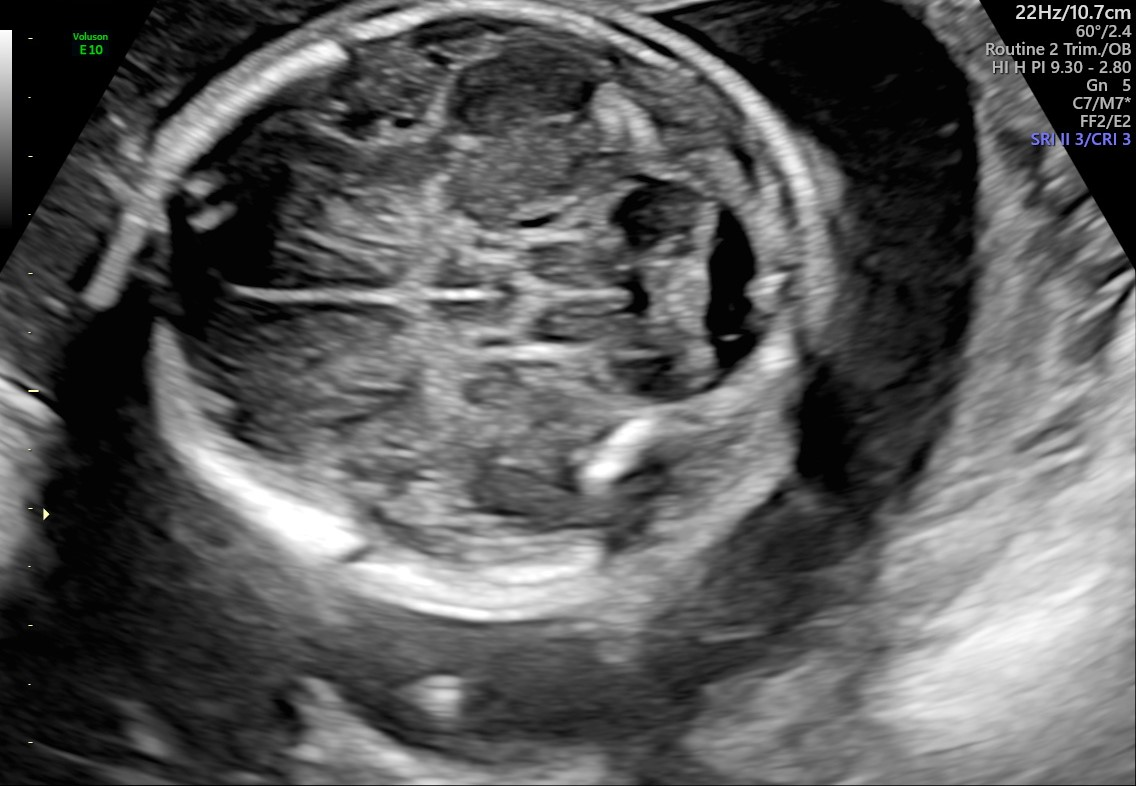
\includegraphics[width= 0.8\textwidth]{img/imagen_cerebelo.jpg} \caption{Ejemplo de ecografía fetal en plano transcerebeloso. Se identifican estructuras anatómicas clave como el vermis cerebeloso, la cisterna magna y los hemisferios cerebelosos.} \label{fig:eco_transcerebeloso} \end{figure} 

A partir de esta necesidad clínica y el avance tecnológico en inteligencia artificial, este proyecto busca desarrollar una herramienta que no solo automatice la segmentación del cerebelo fetal, sino que también facilite su integración en el flujo de trabajo médico habitual. La contribución de este trabajo radica en la propuesta de una solución robusta y escalable, capaz de adaptarse a diversos entornos clínicos y de investigación, sentando las bases para futuras implementaciones en el ámbito del diagnóstico por imagen prenatal. 

De este modo, se pretende contribuir a una atención prenatal más precisa y oportuna, mejorando la calidad del diagnóstico y promoviendo intervenciones tempranas que puedan influir positivamente en el desarrollo neurológico del neonato, siempre teniendo presente que la última palabra en la interpretación diagnóstica corresponde al profesional médico, quien debe evaluar cada caso de forma integral.


\section{Estructura de la memoria}

La memoria se estructura en distintos apartados que recogen tanto los aspectos teóricos como los técnicos y experimentales desarrollados a lo largo del proyecto. Esta organización tiene como objetivo ofrecer una visión clara y progresiva del trabajo realizado, facilitando la comprensión de cada fase del proyecto y su contribución al objetivo global.

\begin{itemize}
    \item \textbf{Introducción}: Contextualiza el problema, resaltando la importancia del análisis del cerebelo fetal en el diagnóstico prenatal y la necesidad de herramientas que mejoren la precisión y eficiencia del proceso. También se incluye una descripción general de la estructura del documento.
    \item \textbf{Objetivos}: Define los objetivos del proyecto, tanto desde el punto de vista técnico como práctico.
    \item \textbf{Conceptos teóricos básicos}: Describe los fundamentos necesarios para entender el proyecto, como los principios del aprendizaje automático y las redes neuronales, así como conceptos relacionados con la anatomía del cerebelo fetal. También se incluye una revisión del estado del arte en segmentación automática aplicada a imágenes médicas.
    \item \textbf{Metodología}: Se detalla el enfoque seguido para el desarrollo del proyecto, incluyendo la estructura del conjunto de datos, el preprocesamiento de imágenes, las técnicas empleadas para el entrenamiento de los modelos y las herramientas utilizadas a lo largo del proceso.
    \item \textbf{Resultados}: Se analizan los modelos entrenados, comparando su rendimiento mediante métricas específicas de segmentación. Se incluyen ejemplos visuales que muestran la segmentación automática en imágenes reales y capturas de la interfaz desarrollada, demostrando su funcionalidad y aplicabilidad práctica.
    \item \textbf{Conclusiones}: Resume los principales hallazgos del proyecto, reflexionando el grado de cumplimiento de los objetivos alcanzados.
    \item \textbf{Líneas futuras de trabajo}: Propone posibles mejoras y ampliaciones que podrían desarrollarse a partir del proyecto actual.
\end{itemize}


\section{Materiales entregados}
Se incorporan a la memoria los anexos, que recogen materiales complementarios que amplían los contenidos desarrollados en el cuerpo principal del trabajo. Los recursos generados a lo largo del proyecto incluyen:
\begin{itemize}
    \item \textbf{Scripts en Python}: código empleado para la preparación del conjunto de datos, el entrenamiento de los modelos de segmentación basados en aprendizaje profundo, las métricas de evaluación y la construcción de una interfaz interactiva para el usuario clínico.
    \item \textbf{Código en LaTeX}: utilizado para la elaboración de la memoria y los anexos.
    \item \textbf{Documentación del proyecto}: incluye tanto la memoria y anexos como otros documentos relevantes, como el proyecto presentado al Comité de ética de Investigación con Medicamentos (CEIM) y las aclaraciones enviadas posteriormente.
    \item \textbf{Resultados}: se recopilan las gráficas y tablas generadas durante la experimentación, que muestran el comportamiento de las arquitecturas evaluadas y sus métricas asociadas.
\end{itemize}

Todo este material se encuentra organizado en el repositorio de GitHub correspondiente al proyecto de segmentación automática del cerebelo fetal, llamado \href{https://github.com/eirarodriguez/fetal_brain_segmentation} {fetal\_brain\_segmentation}.

%\texttt{https://github.com/eirarodriguez/fetal\_brain\_segmentation}.




\capitulo{2}{Objetivos}

Este proyecto tiene como propósito desarrollar un modelo de segmentación de imágenes ecográficas del cerebelo fetal, empleando técnicas de aprendizaje profundo, con la intención de apoyar el análisis médico y mejorar la precisión en el diagnóstico prenatal. A continuación, se detallan los objetivos generales y técnicos que guiarán el desarrollo del proyecto.

\section{Objetivos generales}
\begin{itemize}
    \item Desarrollo de un sistema de segmentación de imágenes ecográficas 2D de cerebelo fetal utilizando técnicas de \textit{Deep Learning}, con el objetivo de apoyar el análisis médico.
    \item Evaluar la precisión y fiabilidad del sistema desarrollado mediante la comparación de distintas arquitecturas y su validación frente a segmentaciones manuales realizadas por el autor, bajo supervisión y aprobación de un experto médico.
    \item Crear una aplicación web que facilite el uso del sistema de segmentación por parte de los profesionales médicos.
\end{itemize}
\section{Objetivos técnicos}
\begin{itemize}
    \item Implementar un sistema de segmentación basado en redes neuronales convolucionales, explorando diferentes arquitecturas dentro del entorno de desarrollo de \textit{Google Colab}.
    \item Aplicar técnicas de preprocesamiento a las imágenes ecográficas 2D para mejorar el desempeño del modelo y reducir el riesgo de sobreajuste.
    \item Validar el sistema utilizando métricas específicas como \texttt{IoU (Intersection over Union)} y realizar ajustes iterativos de los hiperparámetros para optimizar su rendimiento.
    \item Diseñar e implementar una interfaz web funcional que permita cargar imágenes ecográficas y visualizar de forma clara los resultados de segmentación.
    \item Documentar el progreso del desarrollo utilizando repositorios en plataformas como GitHub, favoreciendo la organización del trabajo.
\end{itemize}
\section{Objetivos personales}
Los objetivos a nivel personal son los siguientes:
\begin{itemize}
    \item Profundizar en los conocimientos prácticos adquiridos en el grado (Grado en Ingeniería de la Salud) sobre las técnicas de \textit{Deep Learning}, especialmente aquellas aplicadas a la segmentación de imágenes médicas.
    \item Aprender sobre diferentes modelos de \textit{Deep Learning}, métricas de evaluación y factores que influyen en el proceso de entrenamiento, como los hiperparámetros o la calidad del conjunto de datos.
    \item Familiarizarme con el entorno de desarrollo de \texttt{PyTorch}, aprendiendo a implementar, entrenar y evaluar modelos de segmentación semántica en ecografías 2D.
    \item Adquirir conocimientos sobre la anatomía del cerebelo fetal y comprender la importancia clínica del desarrollo cerebeloso durante el embarazo.
    \item Desarrollar y mejorar la capacidad de documentar y comunicar de forma clara y comprensible los procesos técnicos y resultados obtenidos.
\end{itemize}










\capitulo{3}{Conceptos teóricos}

En este apartado se presentan los conceptos teóricos fundamentales tanto del ámbito tecnológico como biomédico. Además, se incluye una revisión del estado del arte centrada en la segmentación del cerebro fetal mediante técnicas de \textit{deep learning}. 

\section{Inteligencia Artificial y Machine Learning}
\subsection{Inteligencia Artificial}
La Inteligencia Artificial (IA) es una rama de la informática que trata de desarrollar sistemas capaces de realizar tareas que tradicionalmente han requerido inteligencia humana, como el reconocimiento de patrones, la toma de decisiones o la resolución de problemas. Su principal objetivo es dotar a las máquinas de la capacidad de aprender y adaptarse a nuevas situaciones sin intervención humana directa \cite{russell2010ia}.

\subsection{Machine Learning}
El aprendizaje automático o \textit{Machine Learning} (ML) es un subcampo de la IA basado en el desarrollo de algoritmos capaces de aprender a partir de datos. Estos algoritmos identifican patrones y relaciones dentro de los datos para realizar tareas de clasificación, regresión y agrupamiento. Se basan en modelos matemáticos que ajustan sus parámetros internos en función de los ejemplos previamente observados, con el objetivo de generalizar su comportamiento a nuevos casos no vistos \cite{mitchell1997ml}.

En base al tipo de entrenamiento que reciben, los algoritmos de ML se clasifican principalmente en tres categorías \cite{mitchell1997ml}:
\begin{itemize}
    \item \textbf{Aprendizaje supervisado}: el modelo se entrena con un conjunto de datos etiquetados, es decir, cada entrada va acompañada de su salida deseada. 
    \item \textbf{Aprendizaje no supervisado}: el modelo busca estructuras o patrones ocultos entre datos no etiquetados.
    \item \textbf{Aprendizaje por refuerzo}: el sistema aprende a tomar decisiones a través de la iteración con un entorno, optimizando una recompensa acumulada a lo largo del tiempo. 
\end{itemize} 
En el aprendizaje automático tradicional, gran parte del trabajo se centra en el preprocesamiento de los datos y la selección manual de características relevantes, proceso conocido como \textit{feature engineering} \cite{ng2020yearning}. Esta fase puede limitar la capacidad del modelo para reconocer relaciones más complejas en los datos.

\section{Deep Learning}
El aprendizaje profundo o \textit{Deep Learning} (DL) es un área del aprendizaje automático basada en el uso de redes neuronales artificiales con múltiples capas ocultas. Su objetivo es permitir que las máquinas aprendan automáticamente representaciones y patrones complejos a partir de grandes cantidades de datos, sin necesidad de que un programador defina explícitamente las características a extraer.

Una de las principales fortalezas del DL es su capacidad de aprender representaciones jerárquicas de los datos. En sus primeras capas detecta patrones simples, y en capas más profundas combina estas representaciones para identificar conceptos complejos.

La eficacia del DL en los últimos años se ha visto impulsada por la disponibilidad de grandes volúmenes de datos, gracias al \textit{Big Data}, y por el uso de hardware especializado, como \textit{GPUs} (Unidades de Procesamiento Gráfico) o \textit{TPUs} (Unidades de Procesamiento Tensorial), que permiten procesar grandes cantidades de información de manera eficiente \cite{deeplearning2016}. 

\subsection{Segmentación de imágenes}
La segmentación de imágenes es una técnica fundamental en visión por computador. Consiste en dividir una imagen en múltiples regiones o segmentos, donde cada región agrupa píxeles que comparten ciertas características, como color o textura.

Como resultado, permite identificar y aislar objetos o áreas específicas dentro de una imagen, facilitando su análisis automático. 

\subsubsection{Segmentación por instancias}
Este tipo de segmentación no solo clasifica cada píxel con una etiqueta de clase, sino que también diferencia entre distintas instancias de un mismo objeto. Es decir, identifica y separa objetos individuales, incluso si pertenecen a la misma categoría. \cite{klinger2023segmentacion}

En el caso de este proyecto, se emplea este tipo de segmentación, ya que permite que la red neuronal aprenda a delimitarlas con precisión en cada imagen médica, además de clasificar regiones automáticamente. Esto es esencial en aplicaciones clínicas y de diagnóstico.

\section{Redes Neuronales Artificiales}
Las redes neuronales artificiales o \textit{Artificial Neural Networks} (ANN) son modelos computacionales inspirados en el funcionamiento del cerebro humano, en particular, en el modo en que las neuronas del cerebro procesan y transmiten la información \cite{ann2004}. Se diseñan con el objetivo de que aprendan automáticamente, siendo capaces de reconocer patrones, realizar clasificaciones o aproximar funciones no lineales a partir de datos \cite{deeplearning2016}.

Las neuronas artificiales se organizan en capas \cite{ann2004}:
\begin{itemize}
    \item Capa de entrada: recibe los datos de entrada del sistema, como las imágenes.
    \item Capas ocultas: una o varias capas intermedias que procesan información mediante conexiones ponderadas.
    \item Capa de salida: proporciona la respuesta final del modelo, como la máscara de segmentación.
\end{itemize}
Cada conexión entre neuronas tiene asociado un peso que determina la importancia de la señal transmitida. Las neuronas aplican una función de activación a la suma ponderada de sus entradas, lo que introduce no linealidades y permite modelar las relaciones complejas \cite{deeplearning2016}.

El proceso de aprendizaje de estas redes se basa principalmente en dos fases \cite{deeplearning2016}:
\begin{itemize}
    \item \textbf{Propagación hacia adelante (forward propagation)}: los datos se transmiten desde la capa de entrada hasta la salida, generando una predicción.
    \item \textbf{Retropropagación del error (\textit{backpropagation})}: se calcula el error entre la predicción obtenida y la salida deseada, y este error se propaga en sentido inverso a través de la red, actualizando los pesos mediante algoritmos de optimización.
\end{itemize}

A través de múltiples iteraciones de este proceso, la red ajusta sus parámetros internos para mejorar progresivamente su rendimiento y aprender a generalizar a partir de ejemplos.

\subsection{Redes Neuronales Convolucionales (CNN)}
Las redes neuronales convolucionales o \textit{Convolutional Neural Networks} (CNN) son una arquitectura específica de redes neuronales profundas, ampliamente utilizadas para tareas de procesamiento de imágenes, como clasificación, detección de objetos y segmentación \cite{gu2018cnn}. A diferencia de las redes tradicionales, las CNN están diseñadas específicamente para aprovechar la estructura espacial de los datos de entrada, lo que las hace especialmente eficaces en visión por computador \cite{ibmcnn}. 

La CNN típica consta de varias capas, cada una con un propósito específico en el proceso de extracción y aprendizaje de características:  
\begin{itemize}
    \item Capa de convolución: esta capa utiliza filtros o kernels que se deslizan sobre la imagen de entrada para extraer características locales, como bordes, texturas o patrones. Cada filtro está diseñado para responder a características específicas. Se puede destacar que, al aplicar varios filtros, la red aprende a detectar una gran variedad de rasgos relevantes para la tarea \cite{sotil2022cnn}.
    \item Funciones de activación: son funciones no lineales que se aplican a la salida de cada neurona para introducir no linealidad en el modelo, permitiendo así aprender relaciones complejas. Algunas de las funciones más comunes son:
    \begin{itemize}
    \item \texttt{ReLU} (Unidad Lineal Rectificada): activa solo los valores positivos, ayudando a evitar problemas de saturación y acelerando el entrenamiento \cite{ibmcnn}. 
    \item  TanH (Tangente hiperbólica): escala la salida entre -1 y 1, útil en ciertos contextos pero puede sufrir problemas de saturación \cite{deeplearning2016}.
    \item Sigmoide: transforma la salida en un valor entre 0 y 1, especialmente útil para tareas de clasificación binaria, aunque también puede saturarse y ralentizar el aprendizaje \cite{deeplearning2016}.
    \end{itemize}
    \item Capa de Agrupación (Pooling): la función principal de esta capa es reducir la dimensionalidad de las representaciones obtenidas en las capas anteriores, facilitando el manejo de la información y reduciendo el costo computacional. Los dos métodos comunes son \cite{ibmcnn, ajmal2018cnn}:
    \begin{itemize}
        \item Max pooling: selecciona el valor máximo en cada región, conservando las características más importantes.
        \item Average pooling: calcula el promedio de los valores, proporcionando una visión más general de la información en esa región.
    \end{itemize}
\end{itemize}

El flujo jerárquico de las CNN permite que las primeras capas detecten características simples, mientras que las capas más profundas combinan estas representaciones para reconocer estructuras complejas. Esto es especialmente útil en tareas de segmentación médica, donde es necesario identificar con precisión regiones anatómicas específicas dentro de imágenes complejas. 

La Figura \ref{fig:cnn_arquitectura} muestra el flujo jerárquico típico de una CNN, desde la imagen de entrada, pasando por múltiples capas de convolución y agrupación, hasta llegar a una capa completamente conectada que realiza la predicción final.

\begin{figure}[h]
    \centering
    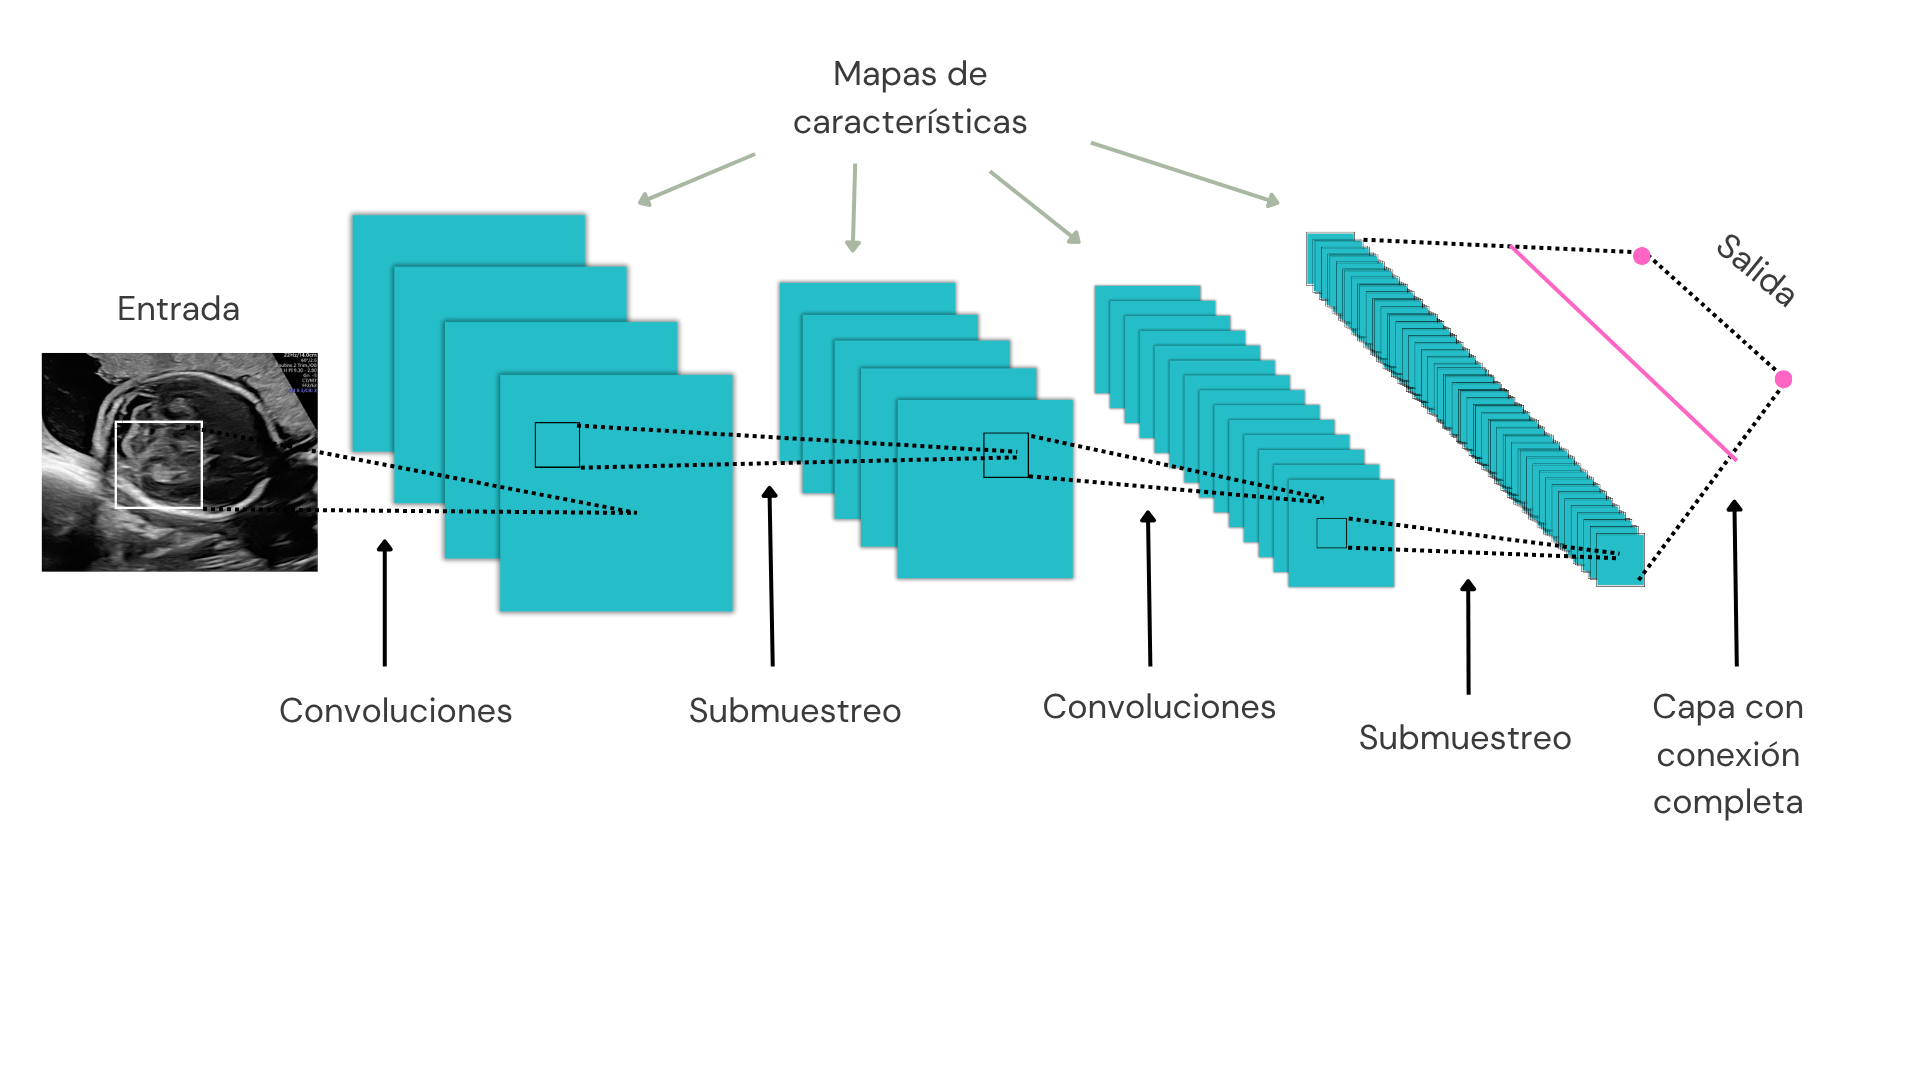
\includegraphics[width= \textwidth]{img/cnn.png}
    \caption{Arquitectura típica de una red neuronal convolucional (CNN). Imagen adaptada de Marcos Esparza Arizpe \cite{cnnimagen}}
    \label{fig:cnn_arquitectura}
\end{figure}

En comparación, las ANN tradicionales utilizan conexiones totalmente conectadas que no distinguen la posición relativa de los datos. Las CNN, en cambio, preservan esta estructura espacial, permitiendo detectar patrones locales específicos. Este enfoque las hace considerablemente más eficaces para tareas como la segmentación de estructuras cerebrales en imágenes fetales \cite{ajmal2018cnn}.


\section{Ecografía}
La ecografía, o ultrasonido médico, es una técnica de imagen que utiliza ondas acústicas de alta frecuencia (normalmente entre 2-10 MHz en diagnóstico fetal) para obtener imágenes de las estructuras internas del cuerpo humano sin necesidad de procedimientos invasivos. Estas ondas se emiten y reciben como ondas mecánicas longitudinales que se propagan a través de los tejidos, reflejándose en las interfaces entre distintos materiales en función de su impedancia acústica \cite{leigthon2007ultrasound}.

Desde un punto de vista físico, el ultrasonido representa una forma de energía mecánica que se transmite en forma de ondas de compresión y rarefacción. Estas ondas generan oscilaciones en las partículas del medio sin producir un desplazamiento neto, permitiendo así el transporte de energía sin transferencia de materia. Este principio físico es lo que permite que esta técnica produzca imágenes en tiempo real \cite{leigthon2007ultrasound, ultrasonido}.

Gracias a estas características, se ha convertido en una herramienta ideal para aplicaciones médicas, especialmente en el campo de la obstetricia. Su carácter seguro, no invasivo y en tiempo real la hace fundamental para observar el desarrollo del feto y detectar posibles anomalías durante la gestación \cite{leigthon2007ultrasound}. 

\subsection{Ecografías 2D}
La ecografía bidimensional (2D) es la modalidad más ampliamente utilizada para representar las imágenes obtenidas mediante ultrasonido. En este tipo de ecografía, el transductor genera un barrido, ya sea mecánico o electrónico, de una sección del cuerpo. Las ondas de ultrasonido reflejadas son procesadas para producir una imagen plana que representa un corte transversal de los tejidos analizados \cite{ultrasonido}.

En el contexto del diagnóstico prenatal, las ecografías 2D permiten una visualización detallada de las estructuras anatómicas del feto, entre ellas el cerebro. Estas imágenes son esenciales para evaluar el crecimiento fetal y posibles anomalías estructurales. Además, presentan ventajas como su alta disponibilidad, relativa simplicidad técnica y bajo coste, lo que las hace accesibles para una amplia gama de aplicaciones clínicas \cite{2dultrasound}.

\section {Cerebelo fetal}
El cerebelo presenta un papel fundamental en el desarrollo neurológico, contribuyendo a funciones motoras, cognitivas y emocionales \cite{schmahmann1998cerebellum}. La evaluación de sus estructuras anatómicas resulta crucial para identificar anomalías en su desarrollo. A continuación, se describen las partes clave del cerebelo.
\subsection{Vermis cerebeloso}
El vermis cerebeloso constituye la parte central del cerebelo, encargado de conectar sus dos hemisferios. Es fundamental en el control del equilibrio, la postura y la coordinación motora. Además, está implicado en funciones cognitivas y emocionales debido a sus conexiones con regiones del cerebro como la corteza prefrontal y el sistema límbico \cite{wolf2009vermis}. En la Figura \ref{fig: parte_anatomicas_cerebelo}, el vermis está marcado en color rosa.

Alteraciones en su desarrollo, como la hipoplasia, se asocian a síndromes neurológicos, entre los que destacan el síndrome de Dandy-Walker \cite{dandy2023} y ciertas formas de ataxia.

\subsection{Cisterna magna}
La cisterna magna o cisterna cerebelomodular es la mayor de las cisternas subaracnoideas del sistema nervioso central. Se localiza entre la superficie inferior del cerebelo y facilita la circulación del líquido cefalorraquídeo (LCR), permitiendo su circulación desde el cuarto ventrículo hacia el espacio subaracnoideo que rodea el encéfalo y la médula espinal \cite{patel2023cisternamagna}. En la Figura \ref{fig: parte_anatomicas_cerebelo}, la cisterna aparece en color amarillo.

Alteraciones en su desarrollo, como la dilatación excesiva, pueden asociarse a diversas malformaciones cerebelosas, como el síndrome de Dandy-Walker y la mega cisterna magna. Estas patologías suelen estar interrelacionadas ya que la ausencia de vermis o hipoplasia del vermis cerebeloso puede generar un agrandamiento anómalo del espacio subaracnoideo, dando lugar a una cisterna magna \cite{patel2023cisternamagna}.

\subsection{Hemisferios cerebelosos}
Los hemisferios cerebelosos constituyen las regiones laterales del cerebelo y se encuentran separados por el vermis. Estas estructuras, junto con la cisterna magna, forman parte del plano transcebeloso evaluado en la ecografía prenatal. Cada hemisferio se divide en lóbulos y lobulillos, cuya corteza se organiza en capas que participan en la coordinación motora y el aprendizaje de movimientos \cite{kenhub}. En la Figura \ref{fig: parte_anatomicas_cerebelo}, los hemisferios cerebelosos están marcados en color morado.


Durante el desarrollo fetal, los hemisferios cerebelosos se expanden lateralmente desde los labios rómbicos, formando el cerebelo. Alteraciones en su desarrollo, como la hipoplasia cerebelosa, pueden comprometer la coordinación motora y otras funciones neurológicas \cite{volpecerebelo}.

\begin{figure}[h]
    \centering
    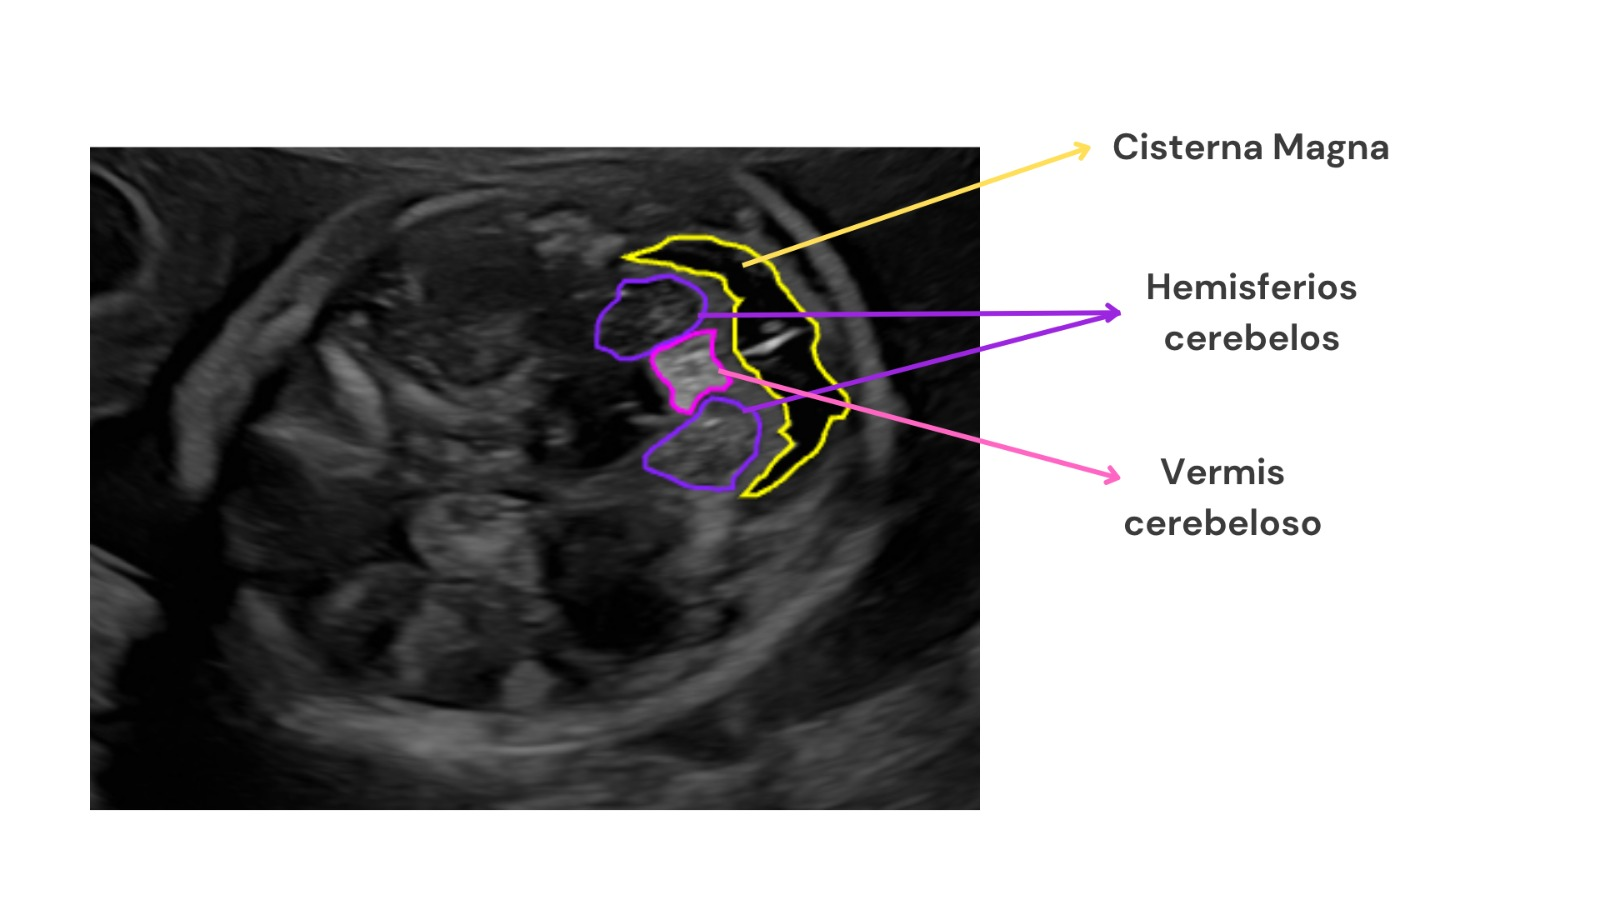
\includegraphics[width=\textwidth]{img/estructuras_interes.jpeg}
    \caption{Localización de las partes claves del cerebelo. Realización propia.}
    \label{fig: parte_anatomicas_cerebelo}
\end{figure}

\section{Estado del arte y trabajos relacionados}
La búsqueda de artículos e investigaciones relacionadas con el proyecto se ha realizado empleando buscadores científicos como \textit{PubMed}, \textit{Google Scholar}, \textit{Web of Science} y \textit{Nature}. A continuación, se exponen los estudios más relevantes encontrados en el ámbito de la segmentación de imágenes médicas mediante técnicas de DL, con especial atención a la aplicación en estructuras cerebrales fetales y análisis de imágenes de ultrasonido.

En el contexto del desarrollo prenatal humano, la detección y análisis temprano de estructuras como el cerebelo fetal es de vital importancia, dada su implicación en el desarrollo neurológico \cite{volpe2009, koning2017impacts}. Para abordar la complejidad inherente a las imágenes de ultrasonido y la variabilidad anatómica, diversos estudios han explorado la aplicación de Redes Neuronales Convolucionales (CNN) y arquitecturas avanzadas de segmentación basadas en DL \cite{hesamian2019}.

A nivel más general, diferentes revisiones han sintetizado los avances más relevantes en el uso de CNN para la segmentación de imágenes médicas \cite{hesamian2019, ajmal2018cnn}. Estos trabajos destacan la eficacia de arquitecturas como U-Net, ampliamente utilizadas por su capacidad para preservar tanto el contexto global como los detalles espaciales en tareas clínicas complejas.

Además, existen ejemplos de aplicación técnica como el presentado por Plain Concepts \cite{plain2021}, donde se describe el uso de modelos inspirados en \texttt{U-Net} para la segmentación precisa de órganos en diversas modalidades de imagen médica. Este tipo de contribuciones demuestra el potencial del aprendizaje profundo en entornos clínicos reales, complementando la evidencia académica.

En conjunto, estos trabajos proporcionan una base sólida para el presente proyecto, al evidenciar los avances en segmentación automatizada y su aplicación específica al análisis de imágenes médicas.


\capitulo{4}{Metodología}

\section{Descripción de los datos}
En este trabajo, las 34 ecografías proporcionadas por el Servicio de Ginecología y Obstetricia del Hospital Universitario de Burgos (HUBU) han servido como base para entrenar las distintas arquitecturas. Los datos fueron divididos en tres subconjuntos: entrenamiento, validación y prueba, con el fin de garantizar una evaluación sólida y evitar el sobreajuste del modelo. En este apartado se describen los datos utilizados.
 
\section{Técnicas y herramientas}
\subsection{Entornos de desarrollo}
\subsubsection{Google Colab}
Google Colab\footnote{Sitio Web de Google Colab: \url{https://cloud.google.com/colab/docs?hl=es-419}} es una plataforma basada en la nube que permite ejecutar notebooks de Jupyter sin necesidad de configuración local. Está especialmente orientada a tareas de ciencia de datos, aprendizaje automático y educación, y ofrece acceso a recursos computacionales como GPUs y TPUs sin coste adicional. 

Los notebooks se almacenan directamente en Google Drive, lo que facilita el acceso desde cualquier lugar y permite la colaboración en tiempo real.

La plataforma es compatible con bibliotecas populares como PyTorch, TensorFlow, pandas y matplotlib, sin necesidad de instalaciones manuales. Permite ejecutar código Python, comandos del sistema e interactuar con el entorno como si fuera local, gracias a máquinas virtuales asignadas automáticamente. Su integración con el ecosistema de Google y su facilidad de uso la convierten en una herramienta ideal para prototipado de modelos de IA.

\subsubsection{Visual Studio Code}
Visual Studio Code \footnote{Sitio Web de Visual Studio Code: \url{https://code.visualstudio.com/}} (VS Code) es un editor de código fuente desarrollado por Microsoft, ampliamente utilizado por su ligereza, rapidez y capacidad de personalización mediante extensiones. En el presente proyecto, se ha utilizado como entorno principal para el desarrollo de la aplicación en Streamlit, permitiendo una edición fluida del código Python, así como la estructuración y prueba del flujo complementario de la herramienta.

Gracias a su integración con Git y GitHub, Visual Studio Code también ha facilitado la subida y gestión del proyecto en repositorios remotos, permitiendo un control de versiones eficiente y una organización clara del trabajo. 

\subsection{Streamlit}
Streamlit\footnote{Sitio Web de Streamlit: \url{https://streamlit.io/}} es un framework de código abierto en Python diseñado para crear aplicaciones web interactivas de forma rápida y sencilla. Su principal ventaja es que permite transformar scripts de Python en interfaces visuales accesibles a usuarios sin conocimientos técnicos.

En este proyecto, Streamlit ha sido utilizado para desarrollar una aplicación interactiva que permite ejecutar el modelo de segmentación sobre ecografías de cerebros fetales, visualizar los resultados de forma clara y descargar un informe en formato PDF con las predicciones generadas, con el fin de facilitar la documentación, el seguimiento clínico y la comunicación de resultados entre profesionales médicos.

Para facilitar su acceso y uso por parte de profesionales médicos o evaluadores externos, la aplicación ha sido desplegada en Streamlit Community Cloud\footnote{Sitio Web de Streamlit Community Cloud: \url{https://streamlit.io/cloud}}, la plataforma gratuita de alojamiento de aplicaciones desarrollada por los propios creadores de Streamlit. Esto ha permitido que la herramienta esté disponible en línea sin necesidad de configuración adicional por parte del usuario final.

\subsection{Lenguajes de programación}
\subsubsection{Python}
Python\footnote{Sitio Web de Python: \url{https://www.python.org/}} es un lenguaje de programación de propósito general, interpretado y de alto nivel, conocido por su sintaxis clara y legible. Esta característica facilita su aprendizaje, convirtiéndolo en una herramienta versátil aplicable en diversos ámbitos como el desarrollo web, la automatización, la ciencia de datos, la IA y el procesamiento de imágenes médicas.

Además, Python ofrece una extensa biblioteca estándar y un amplio ecosistema de paquetes de terceros. Es un lenguaje multiplataforma, de código abierto, respaldado por una comunidad global de desarrolladores que contribuyen de forma constante a su evolución.

En este proyecto, Python ha sido elegido como lenguaje principal debido a su flexibilidad, facilidad de uso y compatibilidad con bibliotecas especializadas en aprendizaje automático y procesamiento de imágenes médicas.
\subsubsection{LaTeX}
LaTeX\footnote{Sitio Web de LaTeX: \url{https://www.latex-project.org/}} es un sistema de preparación de documentos desarrollado sobre el lenguaje tipográfico TeX, orientado principalmente a la creación de textos técnicos y científicos. Su principal ventaja es que permite al autor centrarse en el contenido, mientras que el sistema se encarga automáticamente del formato y la presentación tipográfica.

Gracias a su enfoque basado en comandos estructurados, LaTeX facilita la gestión precisa de bibliografías, ecuaciones, referencias cruzadas, índices, tablas y figuras, ofreciendo resultados de alta calidad tipográfica. 

En el presente proyecto, se ha utilizado este sistema mediante el editor colaborativo Overleaf \footnote{Sitio Web de Overleaf: \url{https://es.overleaf.com/}}, lo que ha permitido una redacción eficiente y organizada del documento.
\subsection{Bibliotecas}
\subsubsection{Procesamiento de Datos y Manipulación de archivos}
\begin{itemize}
    \item \textbf{os} \footnote{Documentación de os: \url{https://docs.python.org/3/library/os.html}} y \textbf{shutil}\footnote{Documentación de shutil: \url{https://docs.python.org/3/library/shutil.html}}: son bibliotecas del módulo estándar de Python utilizadas para interactuar con el sistema de archivos. En este proyecto, \textbf{os} se ha utilizado para gestionar rutas y crea directorios de salida para almacenar resultados, mientras que \textbf{shutil} se ha empleado para mover imágenes entre carpetas, preservando la estructura del conjunto de datos durante el preprocesamiento.
    \item \textbf{pathlib.Path}\footnote{Documentación de pathlib: \url{https://docs.python.org/3/library/pathlib.html}}: \textbf{pathlib}, con su clase \textit{Path}, proporciona una interfaz orientada a objetos para la manipulación de rutas en el sistema de archivos. Se ha utilizado para crear, verificar y manipular rutas de entrada y salida de manera eficiente.
    \item \textbf{pandas}\footnote{Documentación de pandas: \url{https://pandas.pydata.org/docs/}}: es una biblioteca especializada en la manipulación y análisis de datos estructurados, proporcionando estructuras como DataFrame y Series. En este proyecto, se ha usado para organizar y procesar las métricas de evaluación de la segmentación, calcular medias de resultados y preparar las tablas de resultados que posteriormente se exportan como imágenes para su inclusión en los informes finales.
    \item \textbf{NumPy (Numerical Python)}\footnote{Documentación de NumPy: \url{https://numpy.org/doc/}}:es una biblioteca que ofrece estructuras de datos eficientes y un amplio conjunto de funciones para operaciones sobre arrays multidimensionales. En este proyecto, se ha empleado para convertir máscaras de segmentación en arrays numéricos, mapear colores RGB a clases enteras y ejecutar operaciones matriciales de manera rápida, como asignaciones, filtrado o conteo de clases. Esto es esencial para el preprocesamiento de datos y la preparación de entradas para el modelo de aprendizaje profundo.
\end{itemize}
\subsubsection{Procesamiento de imágenes}
\begin{itemize}
    \item \textbf{PIL}\footnote{Documentación de PIL: \url{https://pillow.readthedocs.io/en/stable/}}: a través de su versión moderna \textbf{Pillow}, es una biblioteca de procesamiento de imágenes que permite abrir, editar y guardar archivos de imagen. En el proyecto, se ha utilizado para generar máscaras segmentadas y convertirlas al formato necesario para el modelo.
    \item \textbf{cv2}\footnote{Documentación de OpenCV: \url{https://docs.opencv.org/4.x/index.html}}: correspondiente a OpenCv (Open Source Computer Vision Library), es una herramienta de visión por computador. Aquí se ha empleado para leer imágenes y máscaras, realizar conversiones de espacio de color (como RGB a escala de grises) y preparar los datos visuales para el modelo de segmentación.
\end{itemize}

\subsubsection{Modelado y entrenamiento}
\begin{itemize}
    \item \textbf{torch}\footnote{Documentación de torch: \url{https://docs.pytorch.org/docs/stable/index.html}}: es una biblioteca de código abierto especializada en la computación numérica basada en tensores. En el proyecto, ha servido como base para definir y entrenar el modelo de segmentación.
    \begin{itemize}
    \item \textbf{torch.utils.data}: proporciona herramientas para gestionar conjuntos de datos y facilitar la carga eficiente de datos durante el entrenamiento, organizándolos en batches y simplificando su acceso en cada época.
    \item \textbf{torch.optim.lr\_scheduler}: ofrece métodos para ajustar dinámicamente la tasa de aprendizaje durante el entrenamiento, optimizando la convergencia del modelo. Se ha utilizado para implementar estrategias de aprendizaje adaptativo y mejorar el rendimiento del modelo durante la segmentación.
    \end{itemize}
    \item \textbf{pytorch\_lightning}\footnote{Documentación de pytorch\_lightning: \url{https://lightning.ai/docs/pytorch/stable/}}: es un framework ligero y de alto nivel construido sobre PyTorch que organiza el código de entrenamiento de manera estructural y modular. En este trabajo, ha facilitado la definición de los flujos de entrenamiento, validación y prueba, reduciendo el código repetitivo y mejorando la reproducibilidad de los experimentos.
    \begin{itemize}
    \item \textbf{pytorch\_lightning.callbacks}: incluye herramientas automáticas para gestionar eventos durante el entrenamiento, como la parada temprana (\textit{Early Stopping}) y la monitorización del mejor modelo (\textit{Model Checkpoint}). Estas funciones optimizan el proceso de entrenamiento, asegurando un rendimiento eficiente.
    \end{itemize}
    \item \textbf{segmentation\_models\_pytorch}\footnote{Documentación de segmentation\_models\_pytorch}: \url{https://github.com/qubvel-org/segmentation_models.pytorch?tab=readme-ov-file#api}: es una biblioteca que proporciona implementaciones preentrenadas de modelos avanzados de segmentación de imágenes basados en PyTorch. En este proyecto, se ha utilizado para instanciar arquitecturas competitivas de segmentación, como U-Net++, acelerando el desarrollo y garantizando resultados de alta calidad.
\end{itemize}
\subsubsection{Evaluación y Métricas}
\begin{itemize}
    \item \textbf{scikit-learn}\footnote{Documentación de scikit-learn: \url{https://scikit-learn.org/stable/}}: es una biblioteca de aprendizaje automático que proporciona herramientas eficientes para análisis predictivo y modelado estadístico. En el proyecto se ha utilizado principalmente el siguiente módulo:
    \begin{itemize}
    \item \textbf{sklearn.model\_selection}: ofrece métodos para la división y validación cruzada de conjuntos de datos, optimizando la distribución de los datos en las fases de entrenamiento y evaluación.
    \end{itemize}
    \item \textbf{Matplotlib}\footnote{Documentación de Matplotlib: \url{https://matplotlib.org/stable/index.html}}: es una biblioteca especializada en la generación de gráficos y visualizaciones estáticas, animadas e interactivas. Se ha utilizado para representar resultados de segmentación y visualizar métricas de evaluación de forma gráfica.
    \begin{itemize}
    \item \textbf{matplotlib.pyplot}: proporciona una interfaz sencilla similar a MATLAB para la creación de gráficos. Se ha empleado para visualizar ejemplos de segmentaciones y evolución de métricas de entrenamiento.
    \item \textbf{matplotlib.colors.ListedColormap}: permite definir mapas de colores personalizados, utilizado para representar de forma diferenciada las distintas clases segmentadas en las predicciones del modelo.
    \end{itemize}
\end{itemize}

\subsubsection{Automatización de documentos}
\begin{itemize}
    \item \textbf{python-docx}\footnote{Documentación de python-docx: \url{https://python-docx.readthedocs.io/en/latest/}}: permite crear, modificar y exportar documentos en formato .docx (Microsoft Word) directamente desde Python. Se ha utilizado para automatizar la generación de informes finales, insertando tablas de métricas y resultados de la segmentación de manera estructurada.
\end{itemize}
\subsection{Preprocesamiento de datos}
\subsubsection{Roboflow}
Roboflow\footnote{Página Web de Roboflow: \url{https://docs.roboflow.com/}} es una plataforma integral para el desarrollo de modelos de visión por computador que permite gestionar, anotar, preprocesar y desplegar conjuntos de datos de imágenes. En el contexto del presente trabajo, Roboflow se ha utilizado principalmente para la creación de la \textit{ground truth}.

La herramienta permitió realizar anotaciones manuales mediante segmentación por instancias, utilizando polígonos para delimitar con precisión las estructuras cerebrales de interés. Esto facilitó la creación de máscaras detalladas, necesarias para entrenar modelos de segmentación con alta precisión. 

Además, ha permitido adaptar y modificar los conjuntos de datos según las necesidades del proyecto, ya sea combinando clases, reorganizando anotaciones o generando nuevas versiones conforme aumentaba su volumen. Gracias a sus funcionalidades de gestión y exportación flexible en formatos como COCO, se ha optimizado el flujo de trabajo de preparación de datos, facilitando su integración con entornos de desarrollo basados en PyTorch y PyTorch Lightning.

\subsubsection{Formato COCO}
El formato COCO (Common Objects in Context) es un estándar ampliamente utilizado en visión por computadora para estructurar anotaciones de imágenes en un archivo JSON. Este formato contiene toda la información necesaria para describir las imágenes y sus regiones segmentadas. Entre sus elementos clave se encuentran:
\begin{itemize}
    \item \texttt{categories}: contiene la lista de clases que se utilizan en el dataset. Están definidas con un \texttt{id} numérico y un \texttt{name}.
    \item \texttt{images}: describe las imágenes incluidas en el dataset. Contiene atributos como \textit{id}, \texttt{file\_name} (el nombre del archivo de imagen asociado) y \textit{height} y \texttt{width} (las dimensiones en píxeles de la imagen).
    \item \texttt{annotations}: anotaciones que especifican las regiones segmentadas. Contiene atributos como \texttt{bbox} (la caja delimitadora), \texttt{segmentation}(los puntos que delimitan la región segmentada) y \texttt{category\_id} (la categoría asociada). 
\end{itemize}
Este formato facilita la organización y procesamiento eficiente de datos en proyectos de visión por computadora.
    

\subsection{Herramientas software}
\subsubsection{GitHub}
GitHub\footnote{Página Web de GitHub: \url{https://docs.github.com/es}} es una plataforma de desarrollo colaborativo basada en Git, un sistema de control de versiones distribuido. Permite gestionar proyectos de software mediante repositorios, donde se almacenan, organizan y versionan los archivos. GitHub ha sido una herramienta clave para asegurar el desarrollo eficiente del proyecto, facilitando no solo la organización de tareas y el control de versiones a lo largo del proceso, sino también la creación del repositorio en línea, garantizando el respaldo y acceso remoto al código.
\section{Metodologías}
\subsection{CRISP-DM}
El desarrollo del presente proyecto se guiará por la metodología CRISP-DM (CRoss Industry Standard Process for Data Mining). Esta metodología proporciona un marco estructurado que permite planificar, gestionar y ejecutar proyectos de minería de datos de forma ágil y eficiente, asegurando la trazabilidad y validación en cada una de sus fases \cite{crispdm2021}.

CRISP-DM se compone de seis fases principales, que se desarrollarán de manera iterativa durante el proyecto:
\begin{itemize}
    \item \textbf{Comprensión del negocio (Business Understanding)}: En esta primera fase, se busca comprender en profundidad los objetivos del proyecto, definiendo criterios de éxito y evaluando los recursos disponibles.
    \item \textbf{Comprensión de los datos (Data Understanding)}: Se centra en identificar, recopilar u analizar los conjuntos de datos necesarios para alcanzar los objetivos del proyecto. 
    \item \textbf{Preparación de los datos (Data Preparation)}: Esta etapa incluye todas las tareas necesarias para dejar los datos listos para el modelado.
    \item \textbf{Modelado (Modeling)}: Se aplicarán técnicas de segmentación de imágenes, evaluando distintos algoritmos para determinar cuál ofrece mejores resultados en la detección de estructuras cerebelosas. 
    \item \textbf{Evaluación (Evaluation)}: Se evaluará el rendimiento de los resultados obtenidos para determinar si cumplen con los requisitos clínicos y científicos del proyecto.
    \item \textbf{Implementación (Deployment)}: Finalmente, el modelo será implementado en un entorno funcional, asegurando que sean accesibles y útiles para los interesados.
\end{itemize}
Cada una de estas fases incluirá tareas específicas con un cronograma de ejecución definido, permitiendo un desarrollo progresivo y controlado del proyecto hasta alcanzar los objetivos planteados \cite{crispdm2021}. La Figura \ref{fig:crispdm_diagrama} representa el flujo de trabajo de esta metodología.

\begin{figure}[h]
    \centering
    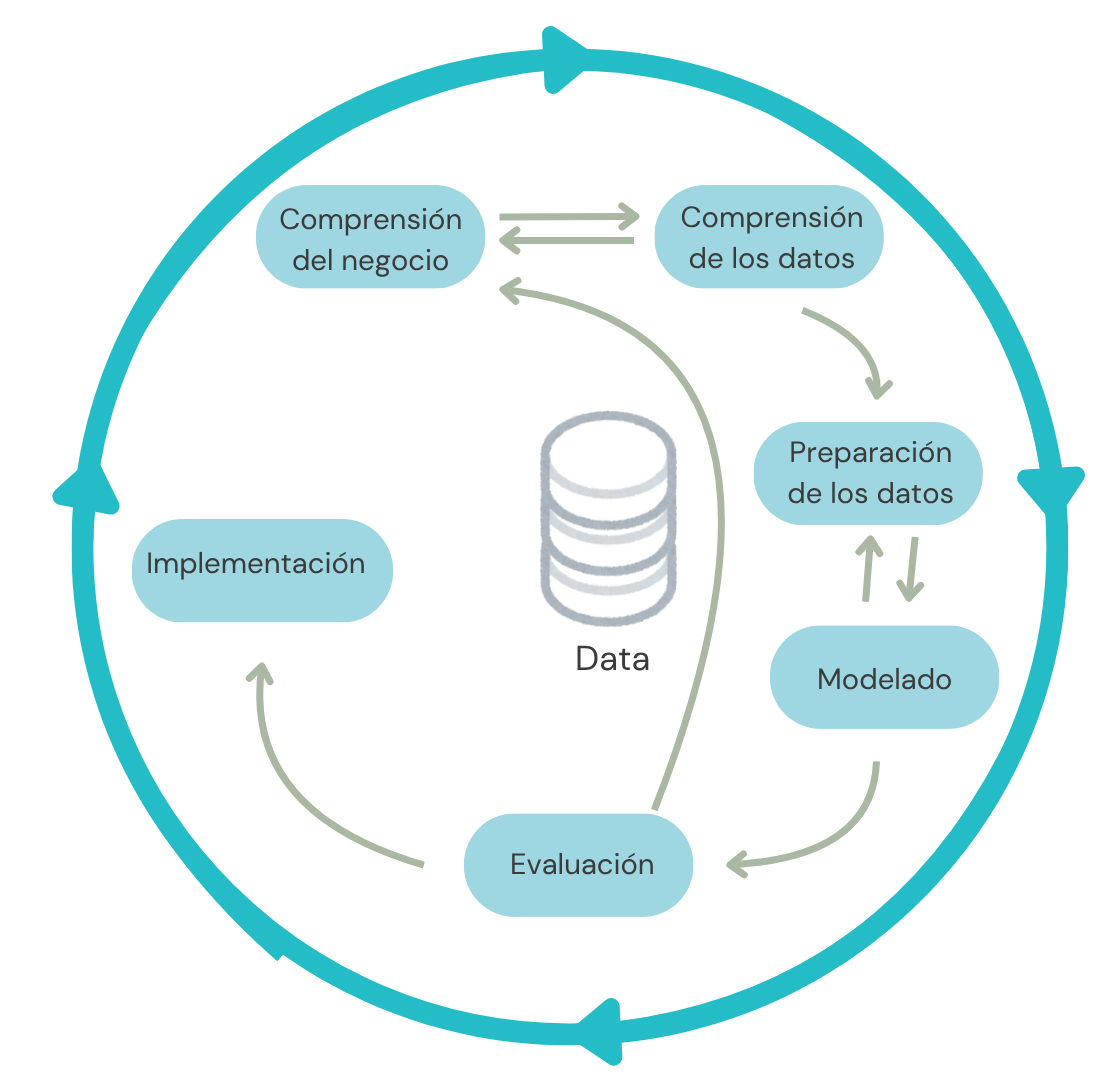
\includegraphics[width= 0.8\textwidth]{img/cripdm_flujo.png}
    \caption{Diagrama del proceso CRISP-DM, adaptado de \cite{crispdmimage}}
    \label{fig:crispdm_diagrama}
\end{figure}

\section{Técnicas}
\subsection{Hold-out}
Una de las técnicas usadas para garantizar que el modelo no solo aprende los datos del conjunto de entrenamiento, sino que también es capaz de generalizar a datos no vistos previamente es el método \textit{hold-out}. Esta técnica consiste en dividir el conjunto de datos disponible en tres conjuntos independientes \cite{deeplearning2016}:
\begin{itemize}
    \item \textbf{Conjunto de entrenamiento (\texttt{train})}: utilizado para ajustar los pesos internos del modelo. Durante esta fase, la red aprende los patrones presentes mediante el proceso de optimización y retropropagación del error (\textit{backpropagation}).
    \item \textbf{Conjunto de validación (\texttt{validation})}: empleado para evaluar el rendimiento del modelo durante el entrenamiento sin influir en el aprendizaje directo. Ayuda a ajustar \textit{hiperparametros} (como la tasa de aprendizaje o el número de capas) y detectar problemas como el \textit{sobreajuste} (\textit{overfitting}).
    \item \textbf{Conjunto de prueba (\texttt{test})}: permite medir el fin de su rendimiento final sobre datos completamente nuevos, y así obtener una estimación objetiva de su capacidad de generalización. 
\end{itemize}

\subsection{Sobreajuste}
El sobreajuste u \textit{overfitting} se produce cuando un modelo se ajusta excesivamente a los datos de entrenamiento, capturando no solo los patrones generales, sino también peculiaridades específicas y ruido inherente de dicho conjunto. Como resultado, aunque el rendimiento del modelo sobre los datos sea excelente, su capacidad para generalizar ante datos nuevos se ve comprometida. 

En términos gráficos, el sobreajuste puede identificarse al observar la pérdida (\textit{loss}) en los conjuntos de entrenamiento y validación. Durante el entrenamiento, la pérdida en el conjunto de entrenamiento disminuye de manera constante. Sin embargo, la pérdida en el conjunto de validación alcanza un punto mínimo y posteriormente comienza a aumentar. Este incremento indica que el modelo está dejando de generalizar y empieza a sobreajustarse, afectando su rendimiento en datos no vistos \cite{ying2019overfitting}.
\subsubsection{Detención temprana}
La técnica de detención temprana o \textit{early stopping} permite prevenir el sobreajuste monitorizando la pérdida en el conjunto de validación durante el entrenamiento. Este método detiene el entrenamiento cuando dicha pérdida alcanza su valor mínimo, ya que se considera que el modelo ha alcanzado su capacidad óptima de generalización. 

Este comportamiento puede visualizarse con claridad a través de las gráficas de pérdida. Al principio, las curvas de entrenamiento y validación descienden juntas, reflejando una mejora general del modelo. No obstante, las curvas pueden divergir, indicando el sobreajuste: la pérdida en el conjunto de entrenamiento continúa disminuyendo, mientras que la del conjunto de validación comienza a incrementarse. Este punto, en el que la pérdida en el conjunto de validación alcanza su valor más bajo antes de aumentar, marca el momento óptimo para aplicar el \textit{early stopping} \cite{ying2019overfitting}.

\begin{figure}[h]
    \centering
    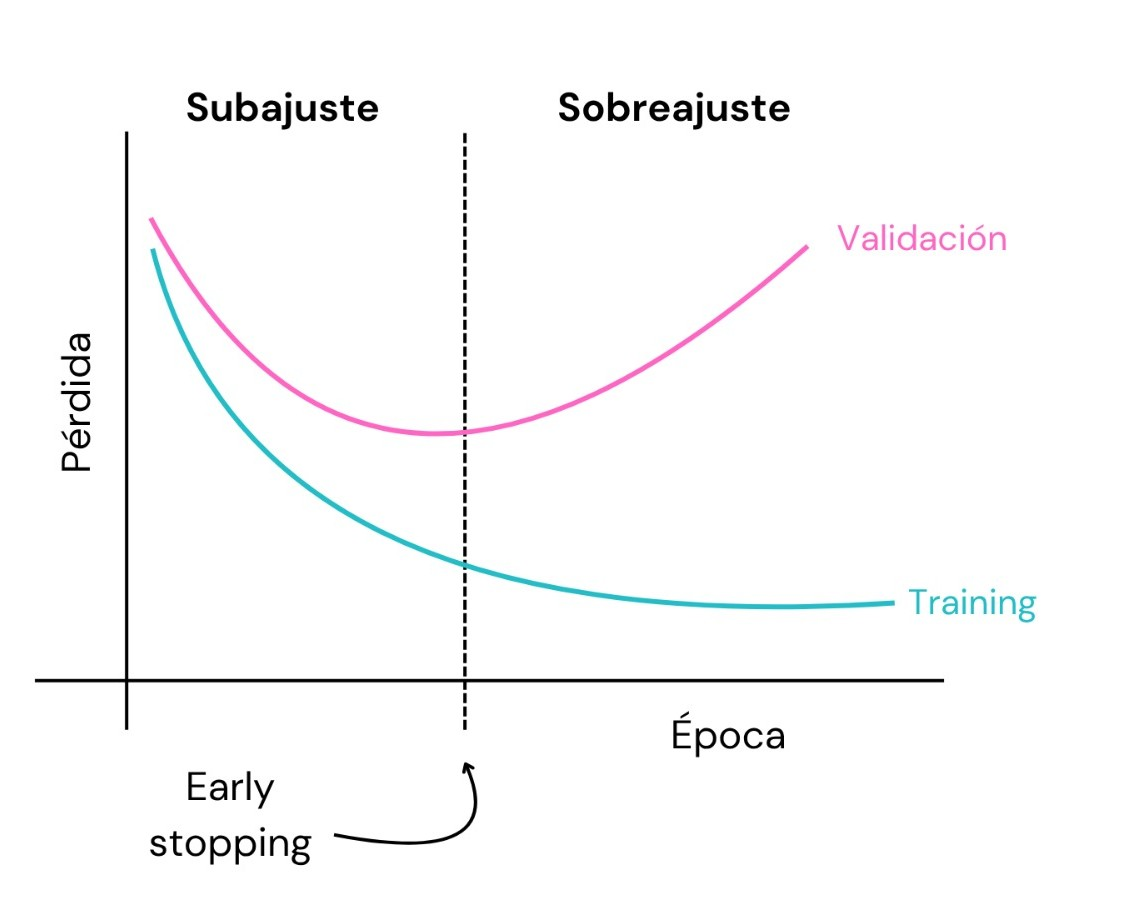
\includegraphics[width= 0.8 \textwidth]{img/early_stopping_grafico.jpeg}
    \caption{Representación gráfica del overfitting y del momento de actuación del early stopping, basada en la explicación gráfica de Holbrook \cite{holbrook2021overfitting}.}
    \label{fig:grafico_overfitting}
\end{figure}

\subsection{Data Augmentation}

El \textit{data augmentation} es una técnica fundamental en aprendizaje profundo que consiste en la generación de nuevas muestras de entrenamiento a partir de transformaciones sobre los datos originales. Estas transformaciones, como rotaciones aleatorias, cambios de escala y ajuste de contraste, permiten aumentar la diversidad del conjunto de datos sin necesidad de recopilar nuevas imágenes \cite{shorten2019da}.

Además, esta técnica contribuye a reducir el sobreajuste y mejorar la capacidad de generalización del modelo, permitiendo que las redes neuronales convolucionales puedan aprender representaciones más robustas incluso cuando se dispone de conjuntos de datos relativamente pequeños, como es el caso en este proyecto \cite{perez2017da}.

\subsection{Métricas de evaluación}
En tareas de segmentación de imágenes médicas, es crucial contar con métricas de evaluación que permitan cuantificar el rendimiento del modelo y garantizar que las predicciones realizadas sean útiles para su aplicación clínica.

\subsubsection{Matriz de confusión}
En el contexto del aprendizaje automático, la matriz de confusión es una herramienta fundamental para evaluar el rendimiento de un modelo de clasificación. Esto permite comparar las predicciones realizadas por el modelo con los valores reales, identificando aciertos y errores en la clasificación \cite{matrizconfusion}, como se ilustra en la Figura \ref{fig:matriz_confusion}.

\begin{figure}[h]
    \centering
    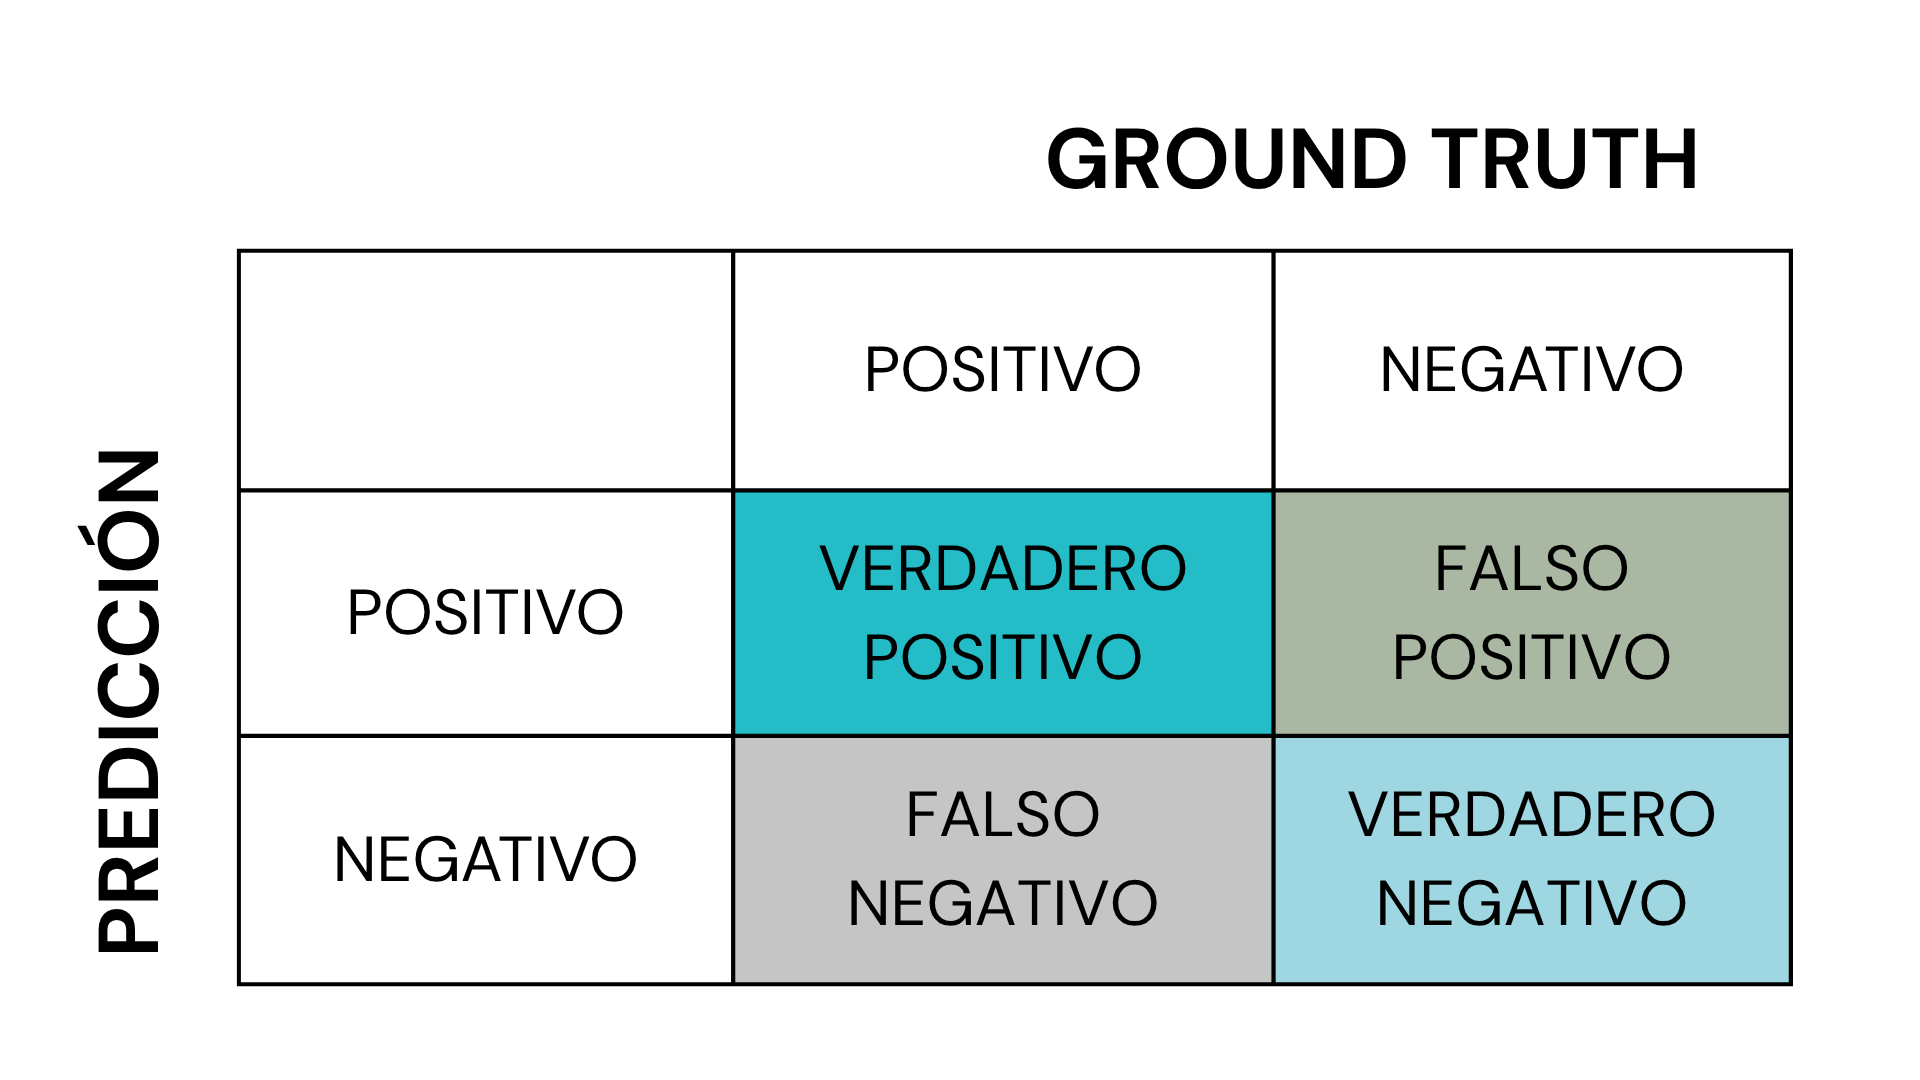
\includegraphics[width= 0.8 \textwidth]{img/matriz_confusion.png}
    \caption{Esquema ilustrativo de la matriz de confusión. Adaptado de \cite{matrizconfusionimage}.}
    \label{fig:matriz_confusion}
\end{figure}
La matriz se organiza habitualmente con las clases reales en las filas y las claves predichas en las columnas. Entre los elementos que la componen destacan los verdaderos positivos (TP), que corresponden a las instancias correctamente clasificadas como positivas, y los falsos positivos (FP), que representan las instancias negativas que el modelo clasificó incorrectamente como positivas. Estos valores permiten calcular la precisión, una métrica clave para interpretar el comportamiento del modelo.

\subsubsection{Precisión}
También conocida como \textit{valor predictivo positivo}, se define como la proporción de TP entre el total de instancias clasificadas como positivas por el modelo, es decir, la suma de TP y FP \cite{Hossin2015precision}. Esta métrica evalúa la exactitud de las predicciones positivas realizadas por el modelo.
Matemáticamente, la precisión se expresa como: 
\begin{equation}
    \text{Precisión} = \frac{TP}{TP+FP}
\end{equation}
\subsubsection{Intersección sobre la Unión}
La métrica Intersección sobre la Unión o Intersection over Union (\texttt{IoU}) o Índice de Jaccard es ampliamente utilizada para evaluar la calidad de segmentaciones en tareas como la segmentación semántica, de instancias y panóptica. Esta métrica calcula la consistencia entre la máscara predicha por el modelo y la máscara de referencia (\textit{ground truth}), considerando todos los píxeles de las áreas segmentadas.

Matemáticamente, se define como:
\begin{equation}
    \text{\texttt{IoU}} = \frac{|P \cap G|}{|P \cup G|}
\end{equation}
donde \textit{P} representa la máscara predicha y \textit{G} la máscara de referencia. Se calculan los píxeles correctamente identificados como pertenecientes a una clase entre los píxeles etiquetados como pertenecientes a la clase de interés. La métrica toma valores entre 0 y 1, donde 1 indica una superposición perfecta. En este trabajo, se calcula un valor de \texttt{IoU} para cada clase segmentada y luego se obtiene la media de estos valores, que corresponde a la media global del rendimiento del modelo de segmentación \cite{cheng2021iou}.




\capitulo{5}{Resultados}

En este capítulo se presentan los resultados obtenidos tras la implementación y evaluación de diferentes arquitecturas de segmentación aplicadas a las estructuras del cerebelo fetal, con el objetivo de analizar y comparar su rendimiento.

\section{Resumen de resultados.}
Durante el desarrollo experimental del proyecto se ha llevado a cabo la implementación de un sistema de segmentación basado en la biblioteca \texttt{segmentation\_models.pytorch}. Se partió de un conjunto de imágenes de ecografías 2D del cerebro fetal en un plano transcerebeloso, proporcionadas por el Servicio de Ginecología del HUBU. 

A partir de estas imágenes se generaron sus máscaras \textit{ground truth}, en las que se anotaron las estructuras anatómicas del cerebelo de interés. Estas máscaras, junto con las imágenes originales, conformaron el conjunto de datos empleado para el entrenamiento de las distintas arquitecturas basadas en redes neuronales convolucionales (CNN). Finalmente, se calcularon diversas métricas de rendimiento que permitieron analizar y comparar el desempeño de cada una de las arquitecturas evaluadas. 

A continuación, se presentan y analizan los resultados obtenidos, comparando diferentes arquitecturas y parámetros, lo cual ha permitido fundamentar la elección del modelo final.

\subsection{Arquitecturas}
\subsubsection{U-Net}
Es una arquitectura tipo \textit{encoder-decoder}, que mediante el uso de abundantes conexiones de salto (\textit{skip connections}), permite combinar el contexto global capturado durante la compresión con los detalles espaciales recuperados en la fase de expansión. Esta integración mejora significativamente la precisión en tareas de segmentación biomédica, al conservar tanto la información contextual como la resolución espacial \cite{unet2015}.
\subsubsection{U-Net++}
\texttt{U-Net++} es una variante de \texttt{U-Net} que introduce una estructura de conectividad más densa entre el codificador y el decodificador. A través de una serie de subdecodificadores intermedios, esta arquitectura refina progresivamente los mapas de características a diferentes profundidades, lo que optimiza la fusión semántica entre escalas y reduce la discrepancia entre las representaciones generadas por el encoder y el decoder \cite{unetplusplus2018}.
\subsubsection{MAnet}
Presenta una arquitectura encoder-decoder similar a \texttt{U-Net}, pero incorpora un módulo de atención múltiple. Este mecanismo permite a la red reforzar dinámicamente la importancia de distintas regiones espaciales y canales de características durante el proceso de reconstrucción. La aplicación jerárquica de esta atención mejora la extracción de características discriminativas, dando como resultado una segmentación más precisa y robusta \cite{manet2020}.
\subsubsection{Linknet}
\texttt{LinkNet} se distingue por la implementación de conexiones directas (\textit{skip connections}) entre los bloques del codificador y sus correspondientes en el decodificador. Estas conexiones permiten reutilizar características previamente extraídas, lo que optimiza la reconstrucción espacial de la imagen y reduce la pérdida de información durante la etapa de codificación \cite{linknet2020}. Como resultado, se obtiene una segmentación eficiente con menor consumo computacional.
\subsubsection{FPN}
La \texttt{FPN} (Feature Pyramid Network) utiliza una estructura piramidal para la fusión de mapas de características a distintas escalas. Mediante una ruta de arriba hacia abajo y conexiones laterales, esta arquitectura mejora la detección y segmentación de objetos de diferentes tamaños \cite{fpnpresentation}.

\begin{figure}[h]
    \centering
    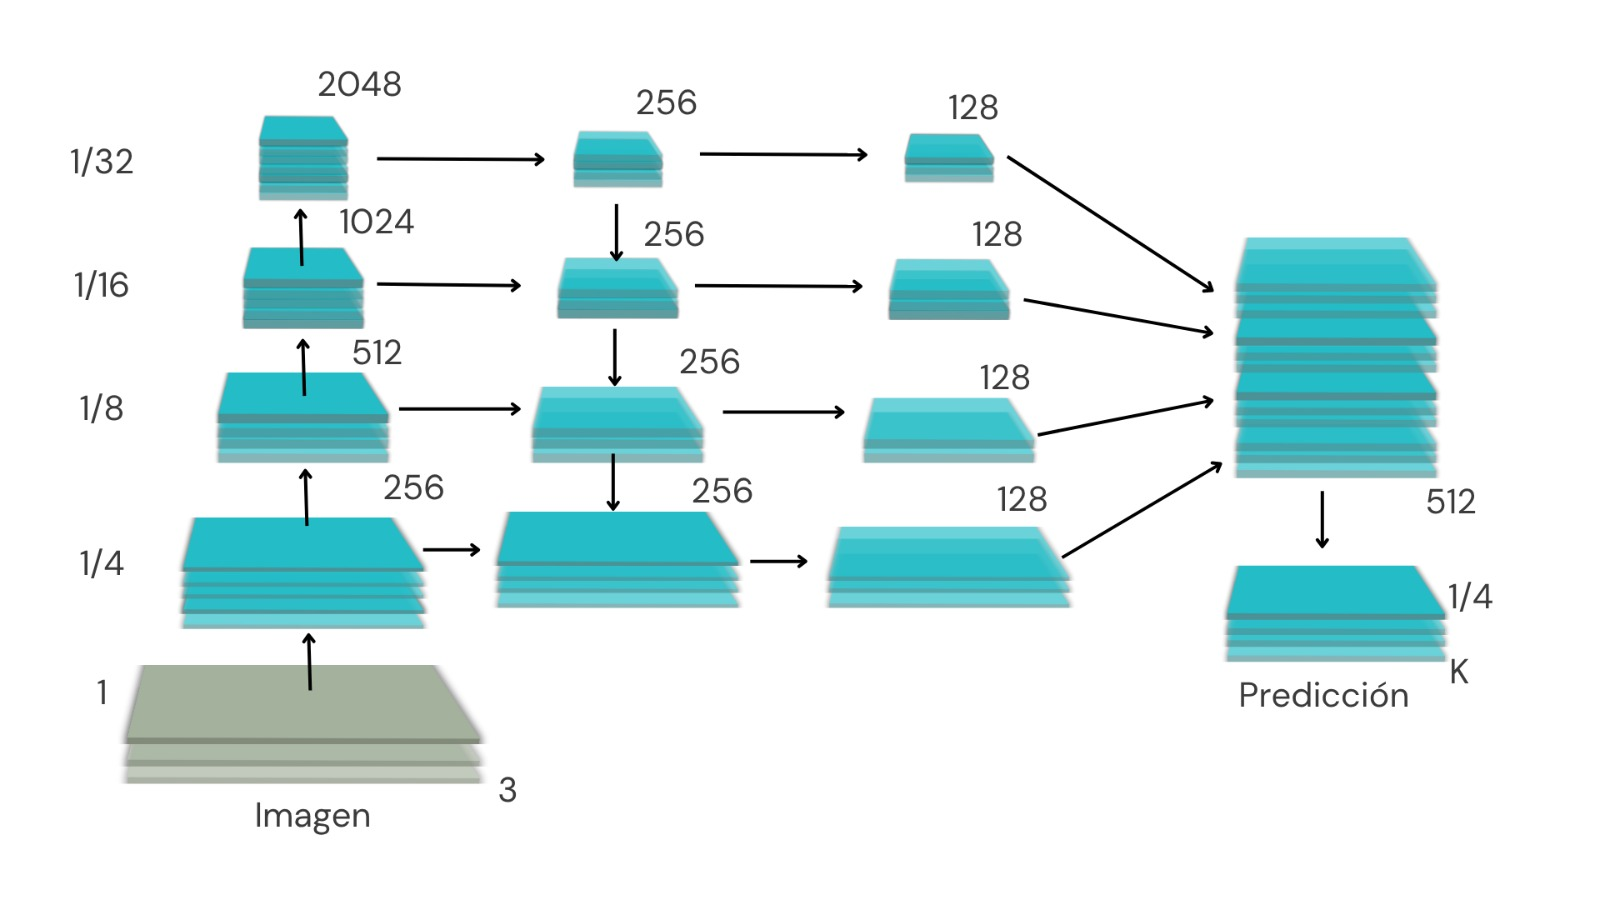
\includegraphics[width= \textwidth]{img/fpn_estructura.jpeg}
    \caption{Esquema de una arquitectura tipo FPN para segmentación semántica. Figura original basada en \cite{fpnpresentation} }
    \label{fig:fpn_diagrama}
\end{figure}

\subsubsection{PSPNet} 
Esta arquitectura introduce un módulo de agrupación piramidal (\textit{pyramid pooling module}), diseñado para capturar información contextual global a múltiples escalas. Este módulo realiza agrupaciones espaciales con diferentes tamaños de ventana sobre el mapa de características, lo que permite a la red integrar tanto contexto global como detalles locales. Gracias a este enfoque, \texttt{PSPNet} es útil en escenarios complejos donde la variabilidad de objetos dificulta una segmentación precisa \cite{pspnet2017}.

Todas las arquitecturas anteriores utilizan el modelo \texttt{resnext50\_32x4d} \footnote{Documentación de resnext50\_32x4d: \url{https://docs.pytorch.org/vision/main/models/generated/torchvision.models.resnext50_32x4d.html}} como encoder preentrenado en \texttt{ImageNet}. Esta arquitectura se basa en el diseño de \texttt{ResNeXt}, incorporando 32 grupos de convoluciones con una anchura de 4. Esto permite mejorar la capacidad de extracción de características sin incrementar significativamente el número de parámetros, lo que hace que sea una opción eficiente para tareas de segmentación.

Para evaluar el rendimiento de estas arquitecturas, se ha realizado un análisis sobre un conjunto de test compuesto por cuatro imágenes. En la Tabla \ref{tab:resultados_sindataaumentation} se presentan los valores medios de precisión e \texttt{IoU} obtenidos en cada arquitectura, destacando la importancia del \texttt{IoU} como métrica fundamental en tareas de segmentación.

\begin{table}[h]
    \centering
    \begin{tabular}{lcc}
    \textbf{Arquitectura} & \textbf{Precisión media (\%)} & \textbf{IoU media (\%)} \\
    \hline
    U-Net             & 49,13 & 45,27\\
    U-Net++           & 49,05 & 45,34\\
    FPN               & 54,08 & 49,88\\
    PSPNet            & 16,56 & 14,75\\
    LinkNet           & 64.05 & 56,83\\
    MAnet             & 55,56 & 43,72\\
    \hfill
    \end{tabular}
    \caption{Comparativa de métricas medias por arquitectura sobre el conjunto de test.} \label{tab:resultados_sindataaumentation}
\end{table}

Con el objetivo de evaluar la robustez del modelo ante variaciones en los datos de entrada, se ha aplicado \textit{data augmentation} sobre el conjunto de test. Las transformaciones utilizadas incluyen rotaciones aleatorias, cambios de escala y ajuste de contraste, con el fin de simular condiciones diversas y mejorar la capacidad de generalización del modelo. La Tabla \ref{tab:resultados_condataaumentation} presenta los resultados obtenidos tras la aplicación de estas técnicas, permitiendo comparar su impacto en la precisión y el \texttt{IoU}.

\begin{table}[h]
    \centering
    \begin{tabular}{lcc}
    \textbf{Arquitectura} & \textbf{Precisión media (\%)} & \textbf{IoU media (\%)} \\
    \hline
    U-Net             & 71,91 & 62,15\\
    U-Net++           & 56,03 & 50,25\\
    FPN               & 59,76 & 54,99\\
    PSPNet            & 17 & 16,53\\
    LinkNet           & 51,77 & 48,22\\
    MAnet             & 56,78 & 35,30\\
    \hfill
    \end{tabular}
    \caption{Comparativa de métricas medias por arquitectura sobre el conjunto de test con data augmentation.} \label{tab:resultados_condataaumentation}
\end{table}

 Tras comparar los resultados obtenidos con y sin \textit{data augmentation}, se observa una mejora generalizada en la mayoría de las arquitecturas, especialmente en la métrica \texttt{IoU}, que resulta la más relevante para la tarea de segmentación. Por tanto, se ha decidido conservar las configuraciones con \textit{data augmentation} como base para la evaluación final.

 Por otro lado, el análisis de las curvas de pérdida durante el entrenamiento reveló indicios de sobreajuste en las arquitecturas, donde la pérdida de validación deja de mejorar o incluso comienza a aumentar tras cierto número de épocas. 

\begin{figure}[h]
    \centering
    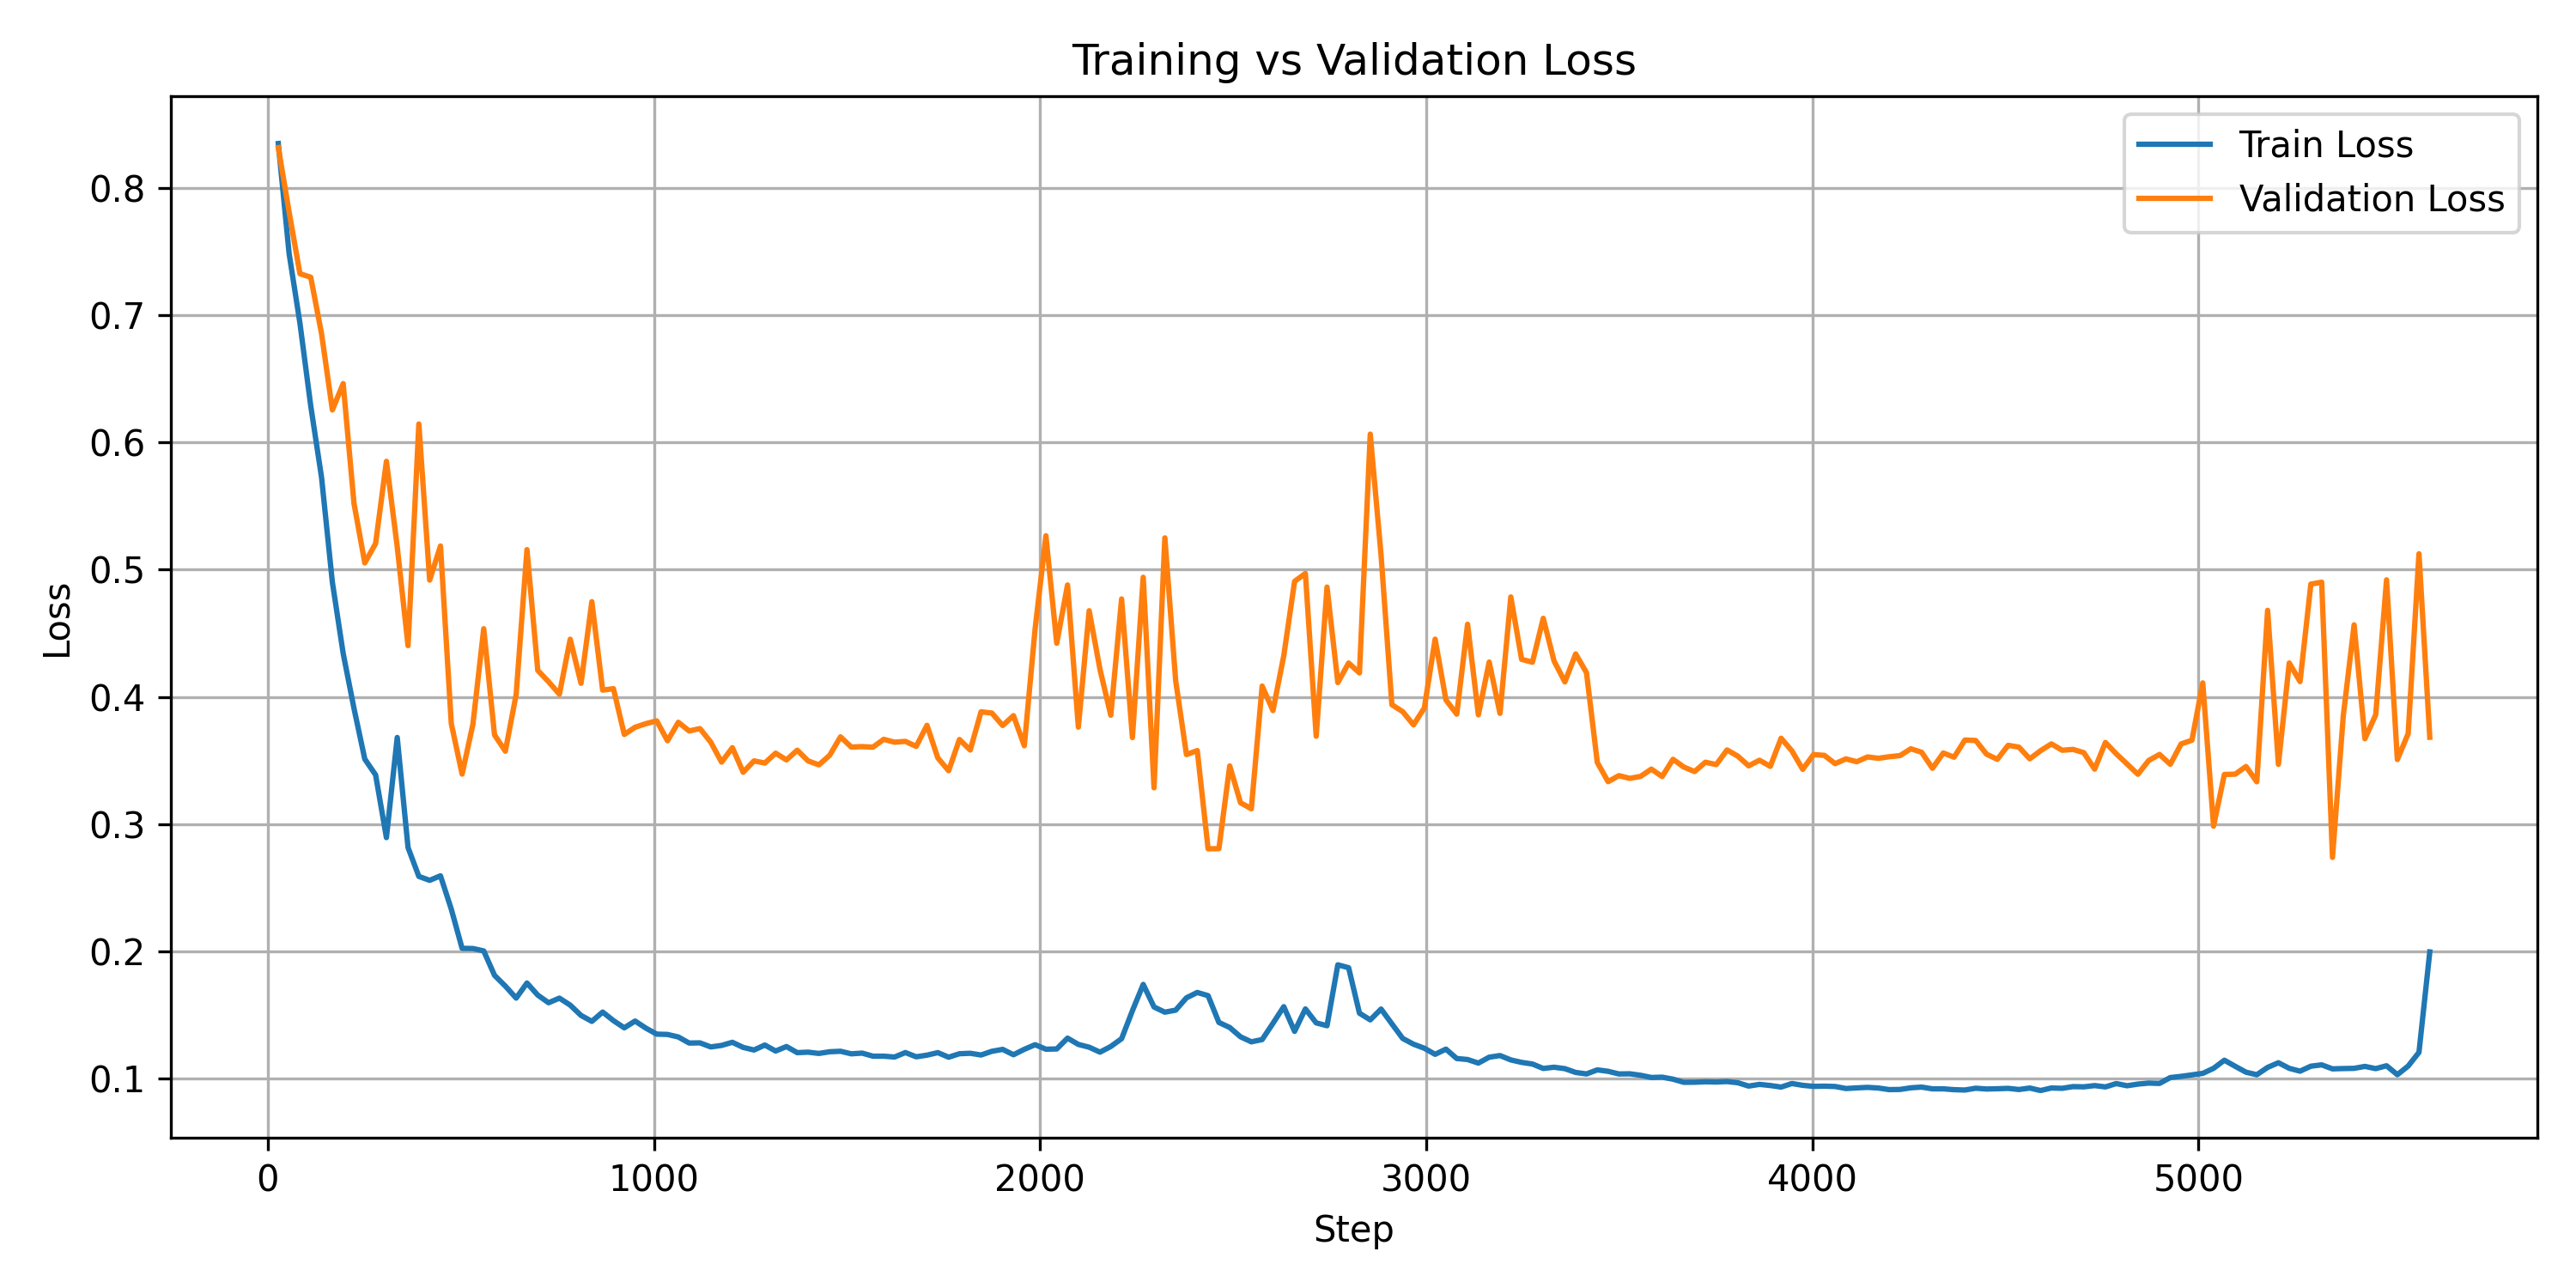
\includegraphics[width= \textwidth]{img/training_vs_validation_loss_manet.png}
    \caption{Curvas de pérdida: MAnet.}
    \label{fig:loss_manet}
\end{figure}

\begin{figure}[h]
    \centering
    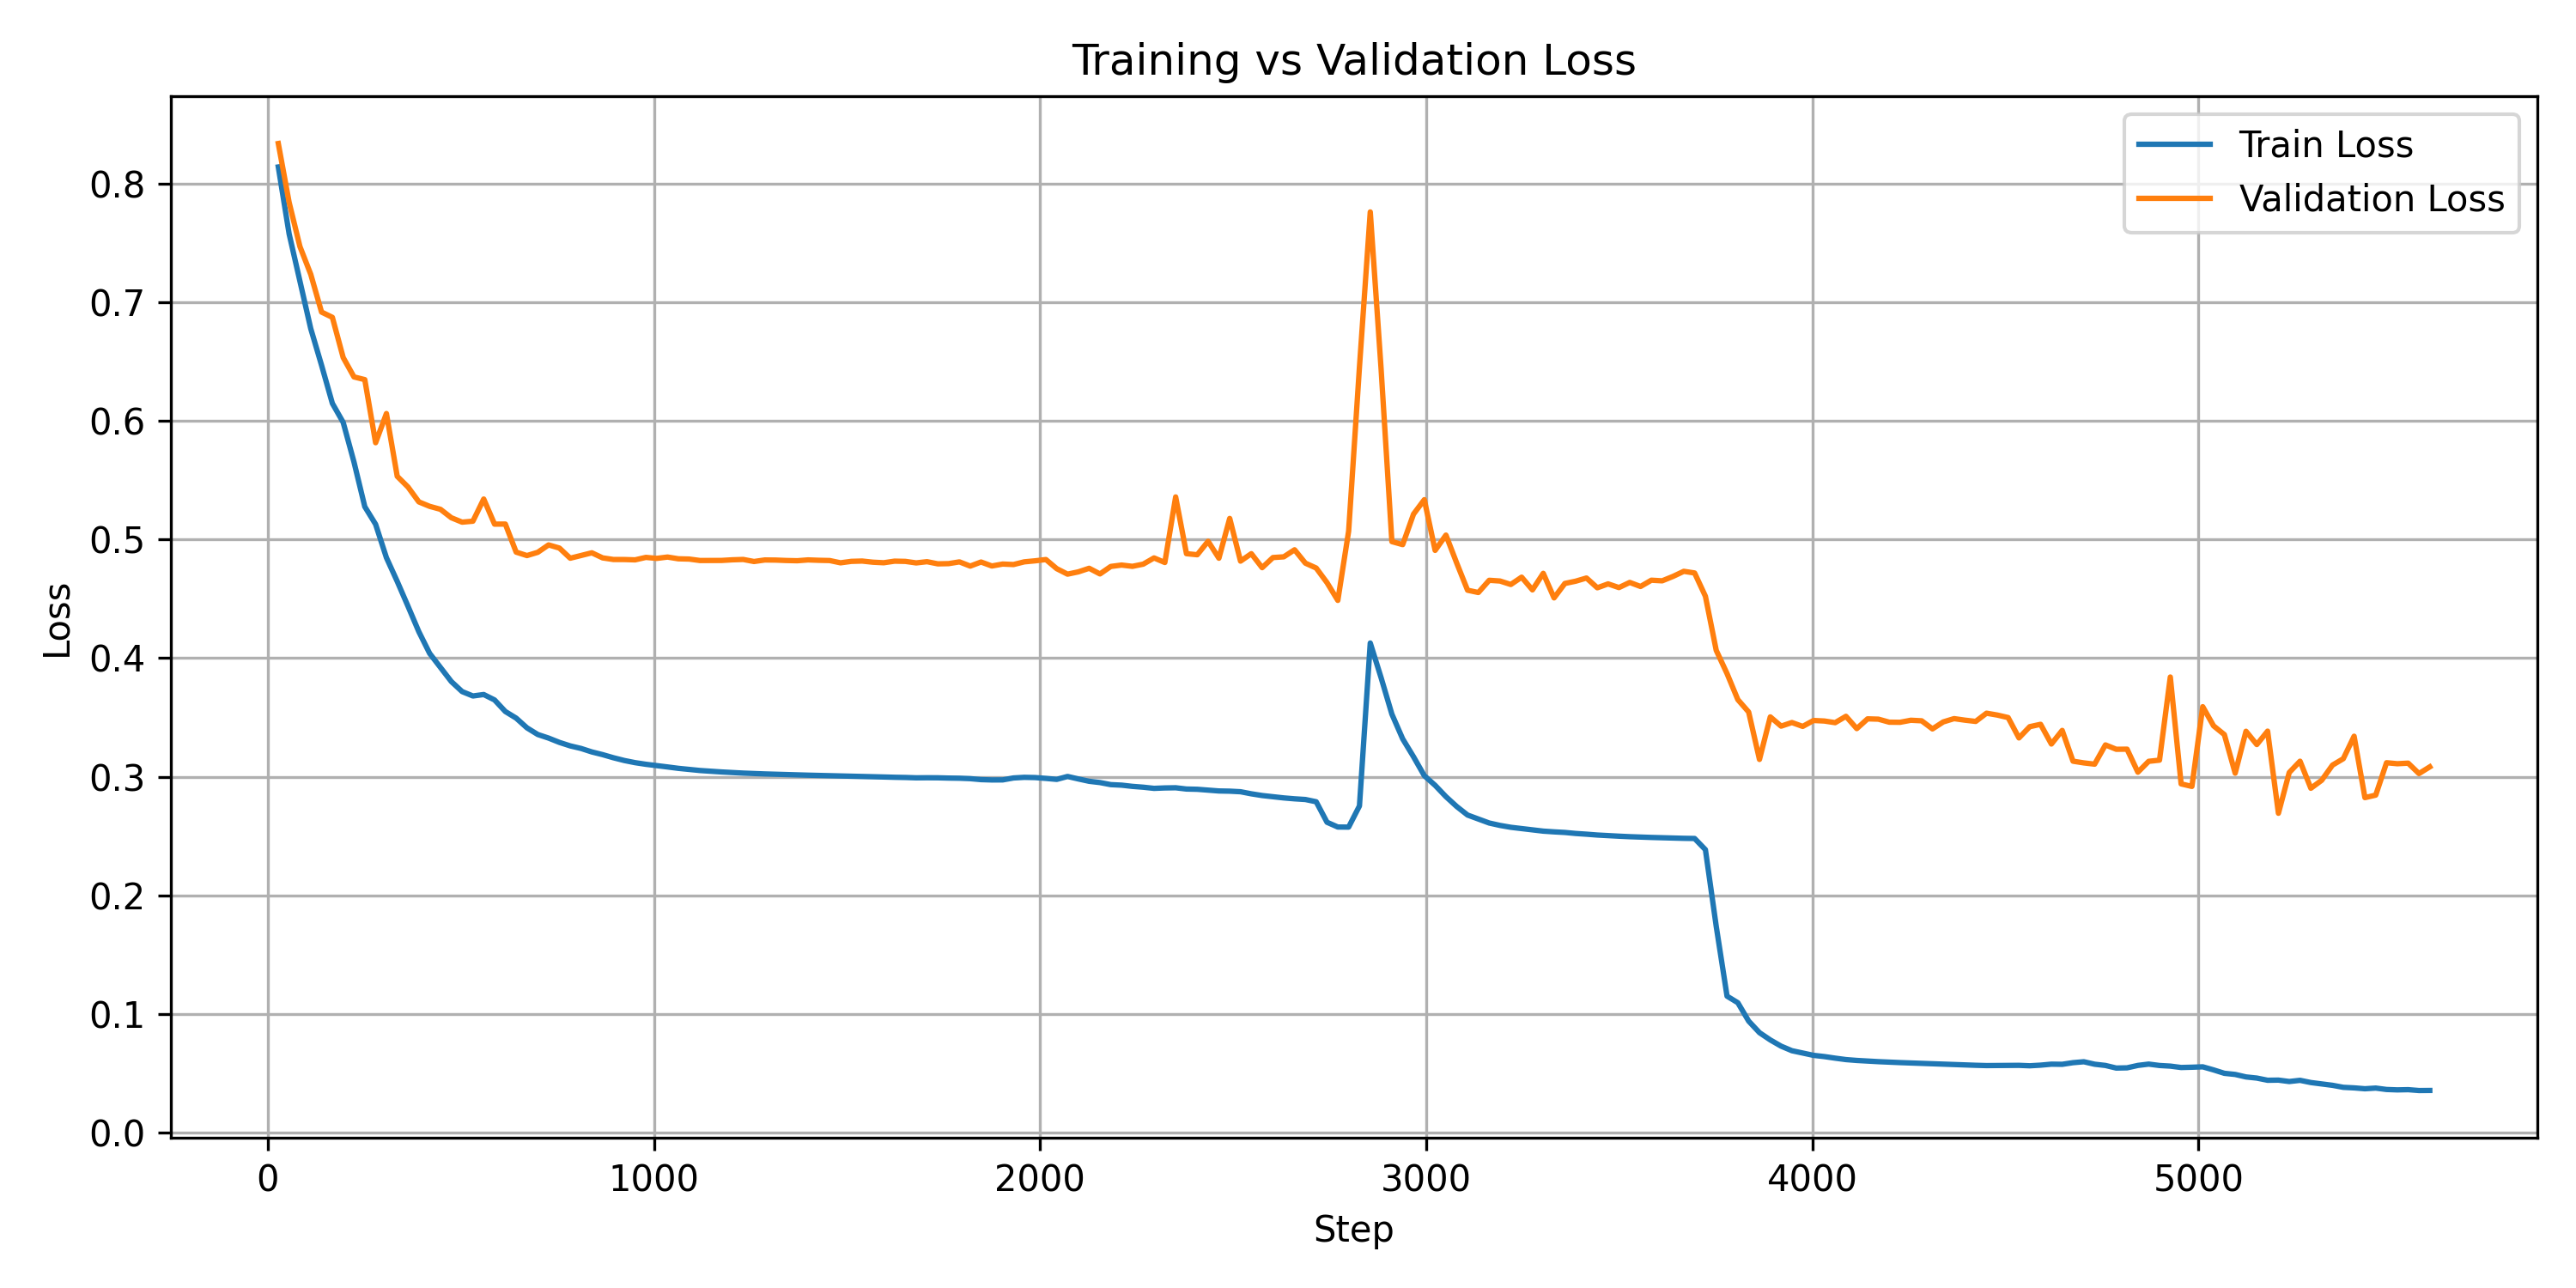
\includegraphics[width= \textwidth]{img/training_vs_validation_loss_unet.png}
    \caption{Curvas de pérdida: U-Net.}
    \label{fig:loss_unet}
\end{figure}

Como se observa en las Figuras \ref{fig:loss_manet} y \ref{fig:loss_unet}, la pérdida de entrenamiento disminuye de forma sostenida, mientras que la de validación tiende a estabilizarse o incluso incrementarse, lo que evidencia el inicio del sobreajuste y justifica la aplicación del criterio de parada anticipada.

Ante esta situación, se incorporó la técnica de \textit{early stopping} como mecanismo de regularización, configurada con una paciencia de 30 épocas sobre la métrica de validación.

\begin{figure}[h]
    \centering
    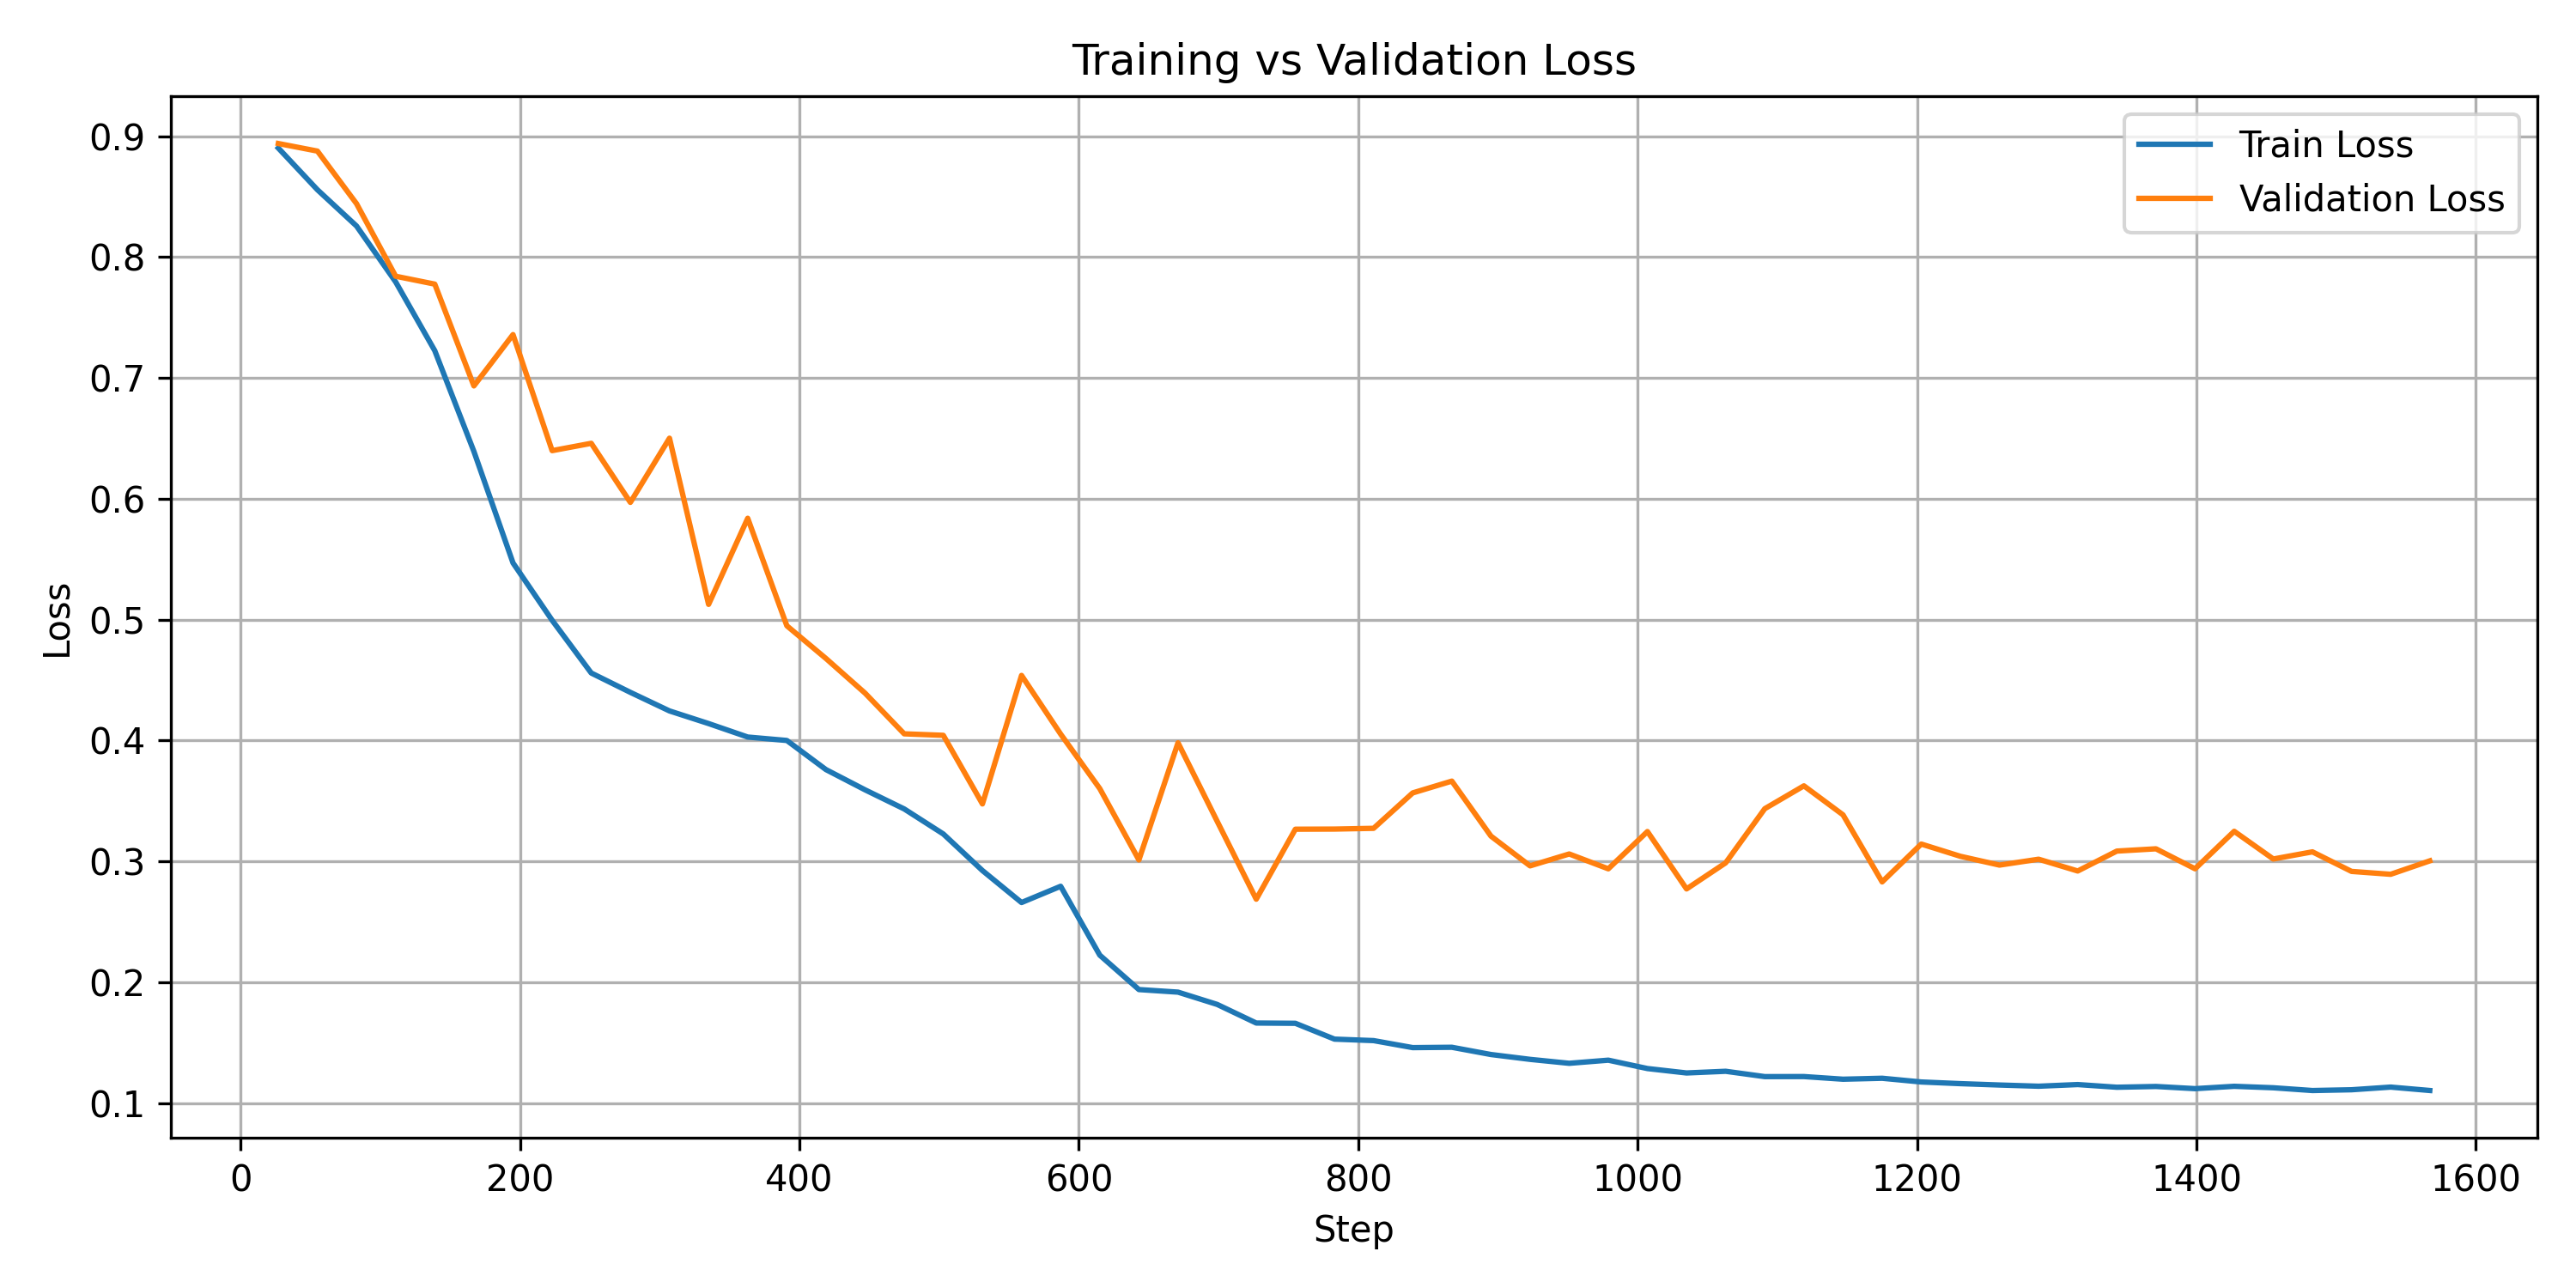
\includegraphics[width=1.1\textwidth]{img/training_vs_validation_loss.png}
    \caption{Curva de pérdida tras aplicar early stopping: U-Net.}
    \label{fig:loss_unet_earlystopping}
\end{figure}

La Figura \ref{fig:loss_unet_earlystopping} muestra un comportamiento específico del entrenamiento de U-Net con \textit{early stopping} activado. Se aprecia cómo el entrenamiento se interrumpe automáticamente al no observarse mejoras sustanciales en la pérdida de validación, lo que contribuye a una mayor eficiencia y generalización del modelo.

En la Tabla \ref{tab:resultados_earlystopping} se muestran los resultados cuantitativos obtenidos en el conjunto de test para cada arquitectura, una vez aplicada la estrategia de regularización.

\begin{table}[h]
    \centering
    \begin{tabular}{lcc}
    \textbf{Arquitectura} & \textbf{Precisión media (\%)} & \textbf{IoU media (\%)} \\
    \hline
    U-Net             & 70.74 & 63,69\\
    U-Net++           & 67,07 & 62,46\\
    FPN               & 70,77 & 60,23\\
    PSPNet            & 15,06 & 12,11\\
    LinkNet           & 71,12 & 60,32\\
    MAnet             & 61,49 & 55,62\\
    \hfill
    \end{tabular}
    \caption{Comparativa de métricas medias por arquitectura sobre el conjunto de test con early stopping.} \label{tab:resultados_earlystopping}
\end{table}

Los resultados muestran un rendimiento competitivo en la mayoría de arquitecturas, destacando LinkNet y FPN en precisión media, mientras que U-Net obtiene la mejor puntuación en \texttt{IoU}. En contraste, PSPNet presenta un rendimiento significativamente inferior, posiblemente debido a una menor capacidad de adaptación al dominio específico del conjunto de datos.

Finalmente, en la Figura \ref{fig:resultado_unet} se muestra un ejemplo representativo de segmentación realizado por U-Net sobre una imagen del conjunto de test. Se puede apreciar una segmentación precisa de las estructuras cerebrales, lo que confirma su capacidad de generalización bajo las condiciones de entrenamiento adoptadas.


\begin{figure}[h]
    \centering
    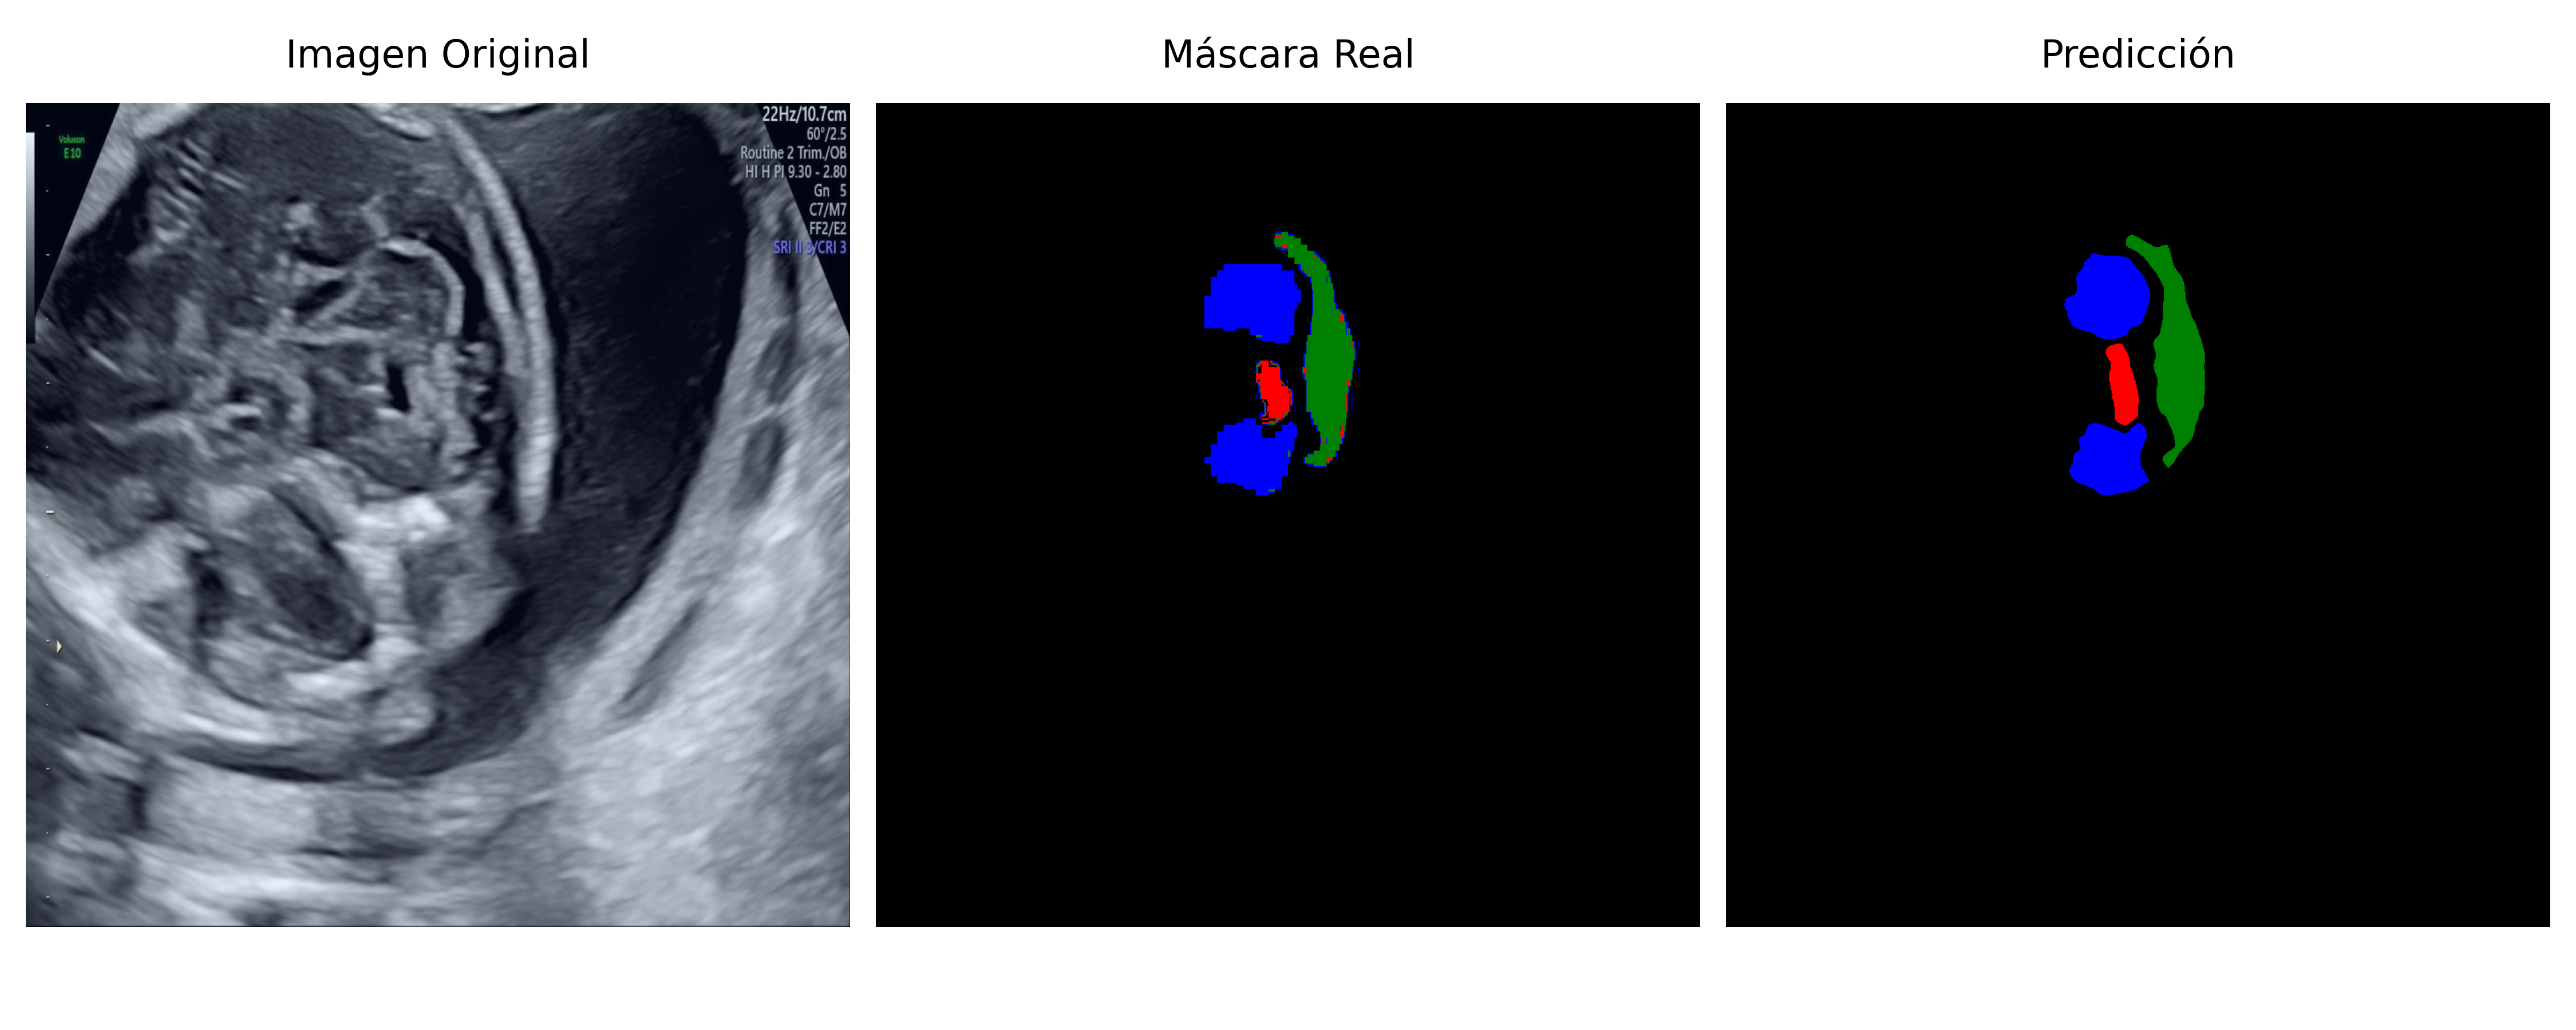
\includegraphics[width=1.1\textwidth]{img/image1_unet.png}
    \caption{Ejemplo de resultado con U-Net. Muestra la imagen original, el resultado de la predicción y la imagen ground truth.}
    \label{fig:resultado_unet}
\end{figure}
 
\section{Discusión.}

Los resultados obtenidos muestran un rendimiento sólido por parte de las arquitecturas evaluadas, destacando especialmente \texttt{U-Net}, que ha alcanzado la mayor puntuación en la métrica \texttt{IoU}. Dado que esta métrica refleja con mayor fidelidad la superposición entre la predicción y la verdad de terreno, se confirma la capacidad del modelo para identificar con precisión las estructuras anatómicas de interés, lo que la posiciona como la opción más adecuada para esta tarea.

La aplicación de \textit{data augmentation} ha demostrado ser una estrategia eficaz para mejorar la generalización. Su incorporación ha derivado en una mejora consistente en las métricas, especialmente en \texttt{IoU}, lo que sugiere que ha compensado adecuadamente la limitada variabilidad presente en el conjunto de datos original. Este resultado refuerza la importancia de emplear técnicas de aumento de datos en escenarios con restricciones muestrales.

Asimismo, la implementación de \textit{early stopping} con una paciencia de 30 épocas ha sido clave para prevenir el sobreajuste. Las curvas de pérdida analizadas evidencian que, sin este mecanismo, la pérdida de validación tiende a estabilizarse o incluso aumentar tras cierto número de épocas, mientras la pérdida de entrenamiento sigue disminuyendo. Este comportamiento es indicativo de un ajuste excesivo al conjunto de entrenamiento, especialmente en arquitecturas más complejas. La incorporación de \textit{early stopping} ha permitido detener el entrenamiento de forma óptima, reduciendo el riesgo de sobreajuste y mejorando la eficiencia computacional.

Respecto al desempeño específico de cada arquitectura, destaca el bajo rendimiento de \texttt{PSPNet}. A pesar de sus buenos resultados en otros dominios, su adaptación al presente escenario ha sido limitada, probablemente por factores como la resolución de las imágenes, el tipo de estructuras o la escasez relativa de los datos. En contraste, modelos como \texttt{LinkNet} y \texttt{FPN} han demostrado un equilibrio entre precisión y capacidad de generalización, posicionándose como alternativas sólidas a \texttt{U-Net}.

Finalmente, los ejemplos cualitativos analizados refuerzan los resultados cuantitativos, mostrando segmentaciones precisas de las principales estructuras cerebrales. Esto confirma que el modelo seleccionado es capaz de extraer representaciones relevantes incluso en un entorno clínico con alta variabilidad anatómica, lo que valida su aplicabilidad práctica. La estabilidad y precisión observada suponen un avance en la automatización del análisis anatómico y abren la puerta a futuras implementaciones en entornos reales de diagnóstico.
\capitulo{6}{Conclusiones}

El presente trabajo ha permitido desarrollar un sistema de segmentación automática de estructuras cerebrales en imágenes médicas fetales, basado en técnicas de aprendizaje profundo. A lo largo del proyecto se han abordado todas las fases necesarias para construir una solución robusta, desde el tratamiento del conjunto de datos hasta el entrenamiento y despliegue del modelo, incluyendo la evaluación cuantitativa y la visualización de resultados.

\section{Aspectos relevantes}

El desarrollo de este proyecto ha supuesto un proceso intensivo de toma de decisiones, resolución de problemas y adquisición de competencias técnicas en distintas áreas del aprendizaje profundo y la ingeniería de software aplicada a imágenes médicas. A continuación, se recogen los aspectos más relevantes y no triviales del trabajo realizado, tanto desde el punto de vista técnico como formativo.

Se ha generado la máscara \textit{ground truth} correspondiente para cada imagen del dataset, codificada en formato multiclase. Este paso ha resultado esencial para garantizar una evolución rigurosa de las predicciones y facilitar el análisis comparativo tanto visual como cuantitativo, lo que resulta especialmente útil en entornos clínicos y docentes. Gracias a esta etapa de procesamiento, se dispone de un conjunto de datos limpio, estructurado y reutilizable, lo cual establece una base sólida para futuras investigaciones.

Uno de los logros más relevantes ha sido la adaptación de un conjunto de datos en formato COCO a un entorno compatible con aprendizaje profundo, generando máscaras segmentadas multicategoría a partir de anotaciones poligonales. Este proceso ha requerido un tratamiento cuidadoso de las clases anatómicas relevantes (cerebelo, cisterna magna y vermis cerebeloso), permitiendo su identificación precisa durante el entrenamiento.

A nivel de arquitectura, se ha evaluado el rendimiento de distintos modelos, siendo \texttt{U-Net} el que ha ofrecido los mejores resultados en términos de \texttt{IoU}, especialmente tras aplicar técnicas de regularización con \textit{data augmentation} y \textit{early stopping}. La integración de estas técnicas ha contribuido significativamente a mejorar la capacidad de generalización del sistema y a prevenir el sobreajuste en entornos de datos limitados, lo cual es habitual en contextos clínicos.

Otro aspecto importante ha sido la implementación del modelo dentro de un entorno profesional con \texttt{PyTorch Lightning}, facilitando la organización del código, el seguimiento de métricas y el uso de estrategias como \textit{ModelCheckpoint} y \textit{segmentation\_models\_pytorch}. También ha permitido acceder a arquitecturas preentrenadas potentes como \texttt{ResNeXt50}, mejorando la precisión del modelo sin necesidad de entrenar desde cero.


Desde una perspectiva práctica, el proyecto culmina con el desarrollo de una aplicación interactiva en \texttt{Streamlit}, que permite cargar imágenes, ejecutar inferencias y visualizar los resultados en tiempo real. Esta herramienta, acompañada de la generación automática de informes médicos en formato PDF, representa un paso real hacia la integración de soluciones de inteligencia artificial en entornos clínicos, orientadas a la mejora del diagnóstico prenatal.

Todo el código ha sido documentado y estructurado para permitir su ejecución reproducible. La segmentación, entrenamiento, validación y visualización están organizadas en módulos separados, lo que facilita tanto su reutilización como su posible ampliación por otros usuarios o investigadores.

Pese a los buenos resultados obtenidos, el proyecto ha puesto en evidencia algunas limitaciones, como la escasez de datos y la dificultad para abordar ciertas estructuras anatómicas de tamaño reducido. Estas limitaciones abren la puerta a futuras líneas de trabajo que permitirían mejorar la precisión, robustez y utilidad clínica del sistema. Entre ellas, se propone aumentar el conjunto de entrenamiento, incorporando mayor variabilidad en las imágenes, así como reconsiderar la inclusión de estructuras como el cuarto ventrículo, cuya segmentación resultó poco precisa en las fases iniciales.

En conjunto, el trabajo ha supuesto una experiencia formativa completa, permitiendo consolidar conocimientos sobre visión por computador, redes neuronales convolucionales y desarrollo de software aplicado al ámbito biomédico. Las técnicas implementadas, los problemas resueltos y las decisiones tomadas durante el proceso representan una base sólida para futuras líneas de investigación y desarrollo en el campo de la imagen médica.

Finalmente, la herramienta desarrollada no solo presenta utilidad clínica, sino también potencial educativo, al permitir la visualización simultánea de la predicción del modelo y la verdad de terreno. Esta capacidad de mostrar errores o aciertos en tiempo real puede ser útil en la formación de personal médico o en la validación cualitativa de modelos.





\capitulo{7}{Lineas de trabajo futuras}

Este capítulo recoge mejoras y extensiones del sistema desarrollado. Se proponen líneas de trabajo orientadas a optimizar el modelo, ampliar el conjunto de datos y reforzar la validación clínica. Estas ideas servirán de base para futuras versiones.

\begin{enumerate}
    \item \textbf{Aumentar el conjunto de datos de entrenamiento:} En este proyecto se ha contado con un total de 34 ecografías, lo cual es una muestra limitada para entrenar un modelo de segmentación robusto y generalizable. Como linea futura, se plantea ampliar el dataset incorporando más imágenes provenientes de diferentes fuentes y con una mayor diversidad de patrones, como ecografías obtenidas en diversos equipos de ultrasonido o en distintas condiciones clínicas. Esto permitiría al modelo capturar mayor diversidad de patrones y mejorar su capacidad para generalizar a nuevos casos.
    \item \textbf{Incorporar la segmentación del cuarto ventrículo:} Inicialmente se exploró la posibilidad de incluir la segmentación del cuarto ventrículo en el modelo. Sin embargo, debido a su tamaño reducido y al desafío asociado a su segmentación precisa, la estructura presentó una precisión cercana a cero en las evaluaciones preliminares. Tras una valoración cuidadosa, se decidió priorizar las estructuras principales del cerebelo, que tienen una mayor relevancia clínica en el contexto del proyecto. Como línea futura, se podría reconsiderar su incorporación si se cuenta con técnicas avanzadas o de un dataset ampliado que mejore la precisión en este tipo de estructuras.
    \item \textbf{Añadir funcionalidades a la aplicación:} se plantea incorporar nuevas funcionalidades que enriquezcan el uso de la herramienta. Por ejemplo, se podría desarrollar una herramienta interactiva para ajustar o refinar los resultados según sea necesario. También sería posible incluir opciones para personalizar parámetros relacionados con el modelo o la visualización, ofreciendo un mayor control sobre el análisis. Además, se podría integrar un módulo de predicción diagnóstica basado en los resultados de segmentación, lo que permitiría extraer conclusiones clínicas automatizadas, aportando un valor significativo para los profesionales médicos y facilitando la toma de decisiones en entornos clínicos.
\end{enumerate}


\bibliographystyle{ieeetr}
\bibliography{bibliografia}


\end{document}
